% ============================================================
%  MindTrace — Final Project Report (Black Book)
%  Main root file — compile this with pdflatex
% ============================================================

\documentclass[12pt, a4paper, oneside]{report}

% ── Encoding & Fonts ────────────────────────────────────────
\usepackage[T1]{fontenc}
\usepackage[utf8]{inputenc}
\usepackage{lmodern}           % Clean scalable fonts

% ── Page Layout ─────────────────────────────────────────────
\usepackage[
  top=1in,
  bottom=1in,
  left=1.25in,
  right=1in
]{geometry}

% ── Line Spacing ────────────────────────────────────────────
\usepackage{setspace}
\onehalfspacing                % 1.5 line spacing throughout

% ── Graphics & Colors ───────────────────────────────────────
\usepackage{graphicx}
\usepackage{subcaption}
\usepackage{float}
\usepackage[dvipsnames]{xcolor}
\graphicspath{{./images/}{./mermaid_diagrams/}}     % graphics search paths
\usepackage{pdfpages}          % embed external PDF pages

% ── Tables ──────────────────────────────────────────────────
\usepackage{booktabs}
\usepackage{longtable}
\usepackage{array}
\usepackage{multirow}
\usepackage{tabularx}

% ── Math ────────────────────────────────────────────────────
\usepackage{amsmath}
\usepackage{amssymb}

% ── Hyperlinks (keep last among most packages) ───────────────
\usepackage[
  colorlinks=true,
  linkcolor=black,
  citecolor=black,
  urlcolor=blue,
  bookmarks=true,
  bookmarksnumbered=true,
  pdftitle={MindTrace - Real-Time Emotion Recognition and Engagement Tracking System},
  pdfauthor={Group XX},
]{hyperref}

% ── Header / Footer ─────────────────────────────────────────
\usepackage{fancyhdr}
\pagestyle{fancy}
\fancyhf{}
\renewcommand{\headrulewidth}{0.5pt}
\renewcommand{\footrulewidth}{0.5pt}
\fancyhead[L]{\small \textit{MindTrace - Real-Time Emotion Recognition and Engagement Tracking System}}
\fancyhead[R]{}
\fancyfoot[L]{\small Dept. of Comp. Engg, PESMCOE Pune}
\fancyfoot[C]{\thepage}
\fancyfoot[R]{\small 2025 - 26}

% Plain style for chapter-opening pages
\fancypagestyle{plain}{%
  \fancyhf{}
  \renewcommand{\headrulewidth}{0pt}
  \fancyfoot[C]{\thepage}
}

% ── Chapter Title Formatting ─────────────────────────────────
% Numbered chapters (Ch.1 onwards): title alone on its own page
% (vertically centred), content starts on the NEXT page.
% Starred chapters (front matter): normal — title at top, content below.
\makeatletter
\renewcommand{\@makechapterhead}[1]{%
  \thispagestyle{plain}%
  \vspace*{\fill}
  {\centering
    \normalfont\Large\bfseries
    CHAPTER \thechapter \\[18pt]
    \Large\MakeUppercase{#1}\par
  }%
  \vspace*{\fill}
  \clearpage
}
% Starred chapters (Certificate, Acknowledgement, Abstract, etc.)
% Title appears at TOP of the page; content follows immediately below.
\renewcommand{\@makeschapterhead}[1]{%
  \thispagestyle{plain}%
  \vspace*{2\p@}%
  {\centering
    \normalfont\Large\bfseries
    \MakeUppercase{#1}\par
  }%
  \vspace{18pt}%
}
\makeatother

% Section / subsection formatting (titlesec for these only)
\usepackage{titlesec}
\titleformat{\section}{\normalfont\large\bfseries}{\thesection}{1em}{}
\titleformat{\subsection}{\normalfont\normalsize\bfseries}{\thesubsection}{1em}{}
\titleformat{\subsubsection}{\normalfont\normalsize\itshape}{\thesubsubsection}{1em}{}

% ── List Formatting ─────────────────────────────────────────
\usepackage{enumitem}

% ── Caption Formatting ──────────────────────────────────────
\usepackage{caption}
\captionsetup{font=small, labelfont=bf}

% ── Code Listings ───────────────────────────────────────────
\usepackage{listings}
\lstset{
  basicstyle=\ttfamily\footnotesize,
  breaklines=true,
  frame=single,
  numbers=left,
  numberstyle=\tiny,
  captionpos=b
}

% ── Miscellaneous ───────────────────────────────────────────
\usepackage{float}             % [H] figure placement
\usepackage{tikz}
\usetikzlibrary{arrows.meta,shapes.geometric,positioning,fit,calc,backgrounds}
\usepackage{subcaption}        % subfigures
\usepackage{parskip}           % space between paragraphs instead of indent
\usepackage{microtype}         % better justification
\usepackage[nottoc,notlof,notlot]{tocbibind} % add Bibliography to TOC

% ============================================================
%  DOCUMENT BEGINS
% ============================================================
\begin{document}

% ── Front Matter (no page numbers / roman numerals) ─────────
\pagenumbering{roman}

% ============================================================
%  TITLE PAGE
% ============================================================
\begin{titlepage}
\centering

\vspace*{0.2cm}

% ── Top label ───────────────────────────────────────────────
{\large \textbf{A PROJECT REPORT ON}}

\vspace{0.2cm}

% ── Project Title ───────────────────────────────────────────
{\Large \textbf{MindTrace: Real-Time Emotion Recognition\\[4pt]
and Engagement Tracking System}}

\vspace{0.2cm}

% ── Submission line ─────────────────────────────────────────
{\normalsize
SUBMITTED TO THE SAVITRIBAI PHULE PUNE UNIVERSITY, PUNE\\
IN THE PARTIAL FULFILLMENT OF THE REQUIREMENTS\\
FOR THE AWARD OF THE DEGREE
}

\vspace{0.25cm}

{\large \textbf{BACHELOR OF ENGINEERING}}\\[2pt]
{\normalsize (\textbf{Computer Engineering})}

\vspace{0.2cm}

{\large \textbf{BY}}

\vspace{0.2cm}

% ── Team Members Table ───────────────────────────────────────
\begin{tabular}{ll}
  Sankalp Gaikwad & B400310457 \\[3pt]
  Hemant Choudhary & B400310444 \\[3pt]
  Shraddha Dashpute & B400310446 \\[3pt]
  Priyanshu Jadhav & B400310472 \\[3pt]
  Balaji Motkulwar & B400310509 \\[3pt]
  
\end{tabular}

\vspace{0.35cm}

{\normalsize \textbf{Under the guidance of}}\\[4pt]
{\normalsize Mrs. Yogita Narwadkar}

\vspace{0.3cm}

% ── College Logo ─────────────────────────────────────────────

\includegraphics[width=2.5cm]{college_logo}

\vspace{0.3cm}

% ── College & University ─────────────────────────────────────
{\large \textbf{DEPARTMENT OF COMPUTER ENGINEERING}}\\[2pt]
{\large \textbf{PES MODERN COLLEGE OF ENGINEERING}}\\[2pt]
{\large \textbf{SHIVAJINAGAR, PUNE 411005}}\\[2pt]
{\large \textbf{SAVITRIBAI PHULE PUNE UNIVERSITY, PUNE}}\\[4pt]
{\large \textbf{2025 - 26}}

\end{titlepage}

% ============================================================
%  CERTIFICATE PAGES
%  Page 1 — Guide & HOD Certificate
%  Page 2 — Completion Certificate (with Examiner signatures)
% ============================================================

% ── Certificate 1: Guide / HOD ──────────────────────────────
\clearpage
\thispagestyle{plain}

\begin{center}

\includegraphics[width=2.5cm]{college_logo}\\[6pt]
{\large \textbf{CERTIFICATE}}
\end{center}

\vspace{0.3cm}

\begin{center}
This is to certify that the Project Entitled
\end{center}

\vspace{0.1cm}

\begin{center}
{\large \textbf{MindTrace: Real-Time Emotion Recognition\\
and Engagement Tracking System}}
\end{center}

\vspace{0.3cm}

\begin{center}
Submitted by
\end{center}

\vspace{0.3cm}

\begin{center}
\begin{tabular}{ll}
  Sankalp Gaikwad & B400310457 \\[4pt]
  Hemant Choudhary & B400310444 \\[4pt]
  Shraddha Dashpute & B40030110446 \\[4pt]
  Priyanshu Jadhav & B400310472 \\[4pt]
  Balaji Motkulwar & B400310509 \\
\end{tabular}
\end{center}

\vspace{0.3cm}

\noindent is a bonafide work carried out by them under the supervision of
\textbf{Mrs. Yogita Narwadkar} and it is approved for the partial fulfillment of the
requirement of Savitribai Phule Pune University, Pune for the award of the
degree of \textbf{Bachelor of Engineering (Computer Engineering)}.

\vspace{1.2cm}

% ── Signature Row ────────────────────────────────────────────
\noindent
\begin{minipage}[t]{0.45\textwidth}
  \centering
  Mrs. Yogita Narwadkar\\[2pt]
  Guide\\[2pt]
  Department of Computer Engineering
\end{minipage}%
\hfill
\begin{minipage}[t]{0.45\textwidth}
  \centering
  Prof.\ Dr.\ Mrs.\ S.\ A.\ Itkar\\[2pt]
  Head\\[2pt]
  Department of Computer Engineering
\end{minipage}

\vspace{2cm}

\noindent
\begin{minipage}[t]{0.45\textwidth}
  \centering
  Signature of Internal Examiner
\end{minipage}%
\hfill
\begin{minipage}[t]{0.45\textwidth}
  \centering
  Signature of External Examiner
\end{minipage}

% ── Certificate 2: Completion Certificate ───────────────────
\newpage
\thispagestyle{plain}

\vspace*{1cm}

\begin{center}
{\normalsize A Project Report on}\\[8pt]
{\large \textbf{MindTrace: Real-Time Emotion Recognition\\
and Engagement Tracking System}}\\[10pt]
{\normalsize is successfully completed by}\\[10pt]
\begin{tabular}{ll}
  Sankalp Gaikwad & B400310457 \\[4pt]
  Hemant Choudhary & B400310444 \\[4pt]
  Shraddha Dashpute & B40030110446 \\[4pt]
  Priyanshu Jadhav & B400310472 \\[4pt]
  Balaji Motkulwar & B400310509 \\[4pt]
\end{tabular}\\[14pt]
{\normalsize at}\\[10pt]
{\large \textbf{DEPARTMENT OF COMPUTER ENGINEERING}}\\[4pt]
{\large \textbf{PES MODERN COLLEGE OF ENGINEERING}}\\[4pt]
{\normalsize SAVITRIBAI PHULE PUNE UNIVERSITY, PUNE}\\[4pt]
{\normalsize \textbf{ACADEMIC YEAR 2025--2026}}
\end{center}

\vspace{2.5cm}

\begin{center}
\begin{tabular}{>{\centering\arraybackslash}p{0.4\textwidth}
                >{\centering\arraybackslash}p{0.4\textwidth}}
  Mrs. Yogita Narwadkar & Prof.\ Dr.\ Mrs.\ S.\ A.\ Itkar \\[2pt]
  Guide        & Head                             \\[2pt]
  Department of Computer Engineering & Department of Computer Engineering \\
\end{tabular}
\end{center}

% ============================================================
%  ACKNOWLEDGEMENT
% ============================================================
\chapter*{Acknowledgement}
\thispagestyle{plain}

It gives us pleasure in presenting the project report on
\textbf{`MindTrace: Real-Time Emotion Recognition and Engagement Tracking System'}.

Firstly, we would like to express our indebtedness appreciation to our guide
\textbf{Mrs.\ Yogita Narwadkar}. Her constant guidance and advice played very
important role in successful completion of the project. She always gave us her
suggestions, that were crucial in making this report as flawless as possible.

We would like to express our gratitude towards \textbf{Prof.\ Dr.\ Mrs.\ S.\ A.\
Itkar}, Head of Computer Engineering Department, PES Modern College of
Engineering for her kind co-operation and encouragement which helped us
during the completion of this report.

Also we wish to thank our Principal, \textbf{Prof.\ Dr.\ Mrs.\ K.\ R.\ Joshi} and
all faculty members for their whole hearted co-operation for completion of
this report. We also thank our laboratory assistants for their valuable help
in laboratory.

Last but not the least, the backbone of our success and confidence lies solely
on blessings of dear parents and lovely friends.

\begin{flushright}
\begin{tabular}{l}
  Sankalp Gaikwad \\[6pt]
  Hemant Choudhary \\[6pt]
  Shraddha Dashpute \\[6pt]
  Priyanshu Jadhav \\[6pt]
  Balaji Motkulwar \\
\end{tabular}
\end{flushright}

% ============================================================
%  ABSTRACT
% ============================================================
\chapter*{Abstract}
\thispagestyle{plain}

Real-time emotion recognition and engagement tracking in educational and professional environments remains a significant challenge, as traditional assessment methods are subjective and impractical at scale. \textbf{MindTrace} addresses this by providing a fully automated system that operates through a standard webcam without any additional hardware. It uses \textbf{MediaPipe Face Mesh} for face detection, feeding regions into a \textbf{ResNet-18} model fine-tuned on the \textbf{RAF-DB} dataset to classify seven emotional states: \textit{Angry, Disgust, Fear, Happy, Neutral, Sad,} and \textit{Surprise}. A composite engagement score (0--100) is computed by combining the detected emotion, head pose estimation, and blink-rate analysis.

The backend is built on \textbf{FastAPI} following a stateless, client-driven architecture where individual webcam frames are sent via REST endpoints for inference, enabling seamless cloud deployment on \textbf{Hugging Face Spaces} without dependency on local hardware. All session data, emotion logs, and engagement metrics are persisted in a \textbf{MongoDB} database to support historical analytics and reporting. The \textbf{React} frontend delivers a professional analytics dashboard featuring live emotion overlays, session timelines, emotion distribution charts, and a multi-user admin panel. Security is handled through \textbf{JWT}-based authentication and \textbf{bcrypt} password hashing with role-based access control for students and administrators. The ResNet-18 model achieves over \textbf{85\%} validation accuracy on the RAF-DB benchmark, and the overall system demonstrates low-latency real-time performance suitable for deployment in e-learning platforms, corporate training environments, and remote work settings.

% ── Keywords ────────────────────────────────────────────────
\newpage
\chapter*{Keywords}
\thispagestyle{plain}

\noindent
Emotion Recognition, Facial Action Units, ResNet-18, RAF-DB Dataset,
MediaPipe Face Mesh, Head Pose Estimation, Engagement Tracking, FastAPI,
MongoDB, React, JWT Authentication, Deep Learning, Transfer Learning,
Real-Time Processing, Student Engagement


% ── Table of Contents / Figures / Tables ────────────────────
% Each starts on its own fresh page
\clearpage
\tableofcontents
\clearpage
\listoffigures
\clearpage
\listoftables

% ── Main Matter (Arabic page numbers from Introduction) ─────
\cleardoublepage
\pagenumbering{arabic}

% ============================================================
%  CHAPTER 1 — INTRODUCTION
% ============================================================
\chapter{Introduction}

\section{Motivation}

The rapid shift toward remote learning, online education, and digital workplaces
has created an urgent need for tools that can objectively measure learner and
employee engagement. In a traditional classroom or meeting room, an instructor or
manager can intuitively observe whether participants are attentive, confused,
frustrated, or simply disengaged. However, in virtual environments — or even
large physical classrooms — such qualitative assessment becomes impractical at
scale.

Research consistently shows that emotional state is one of the strongest
predictors of learning outcomes and work productivity. A student experiencing
confusion or frustration is likely to disengage if not promptly supported,
while a student expressing curiosity or happiness is more likely to retain
information. Despite this, most e-learning and remote work platforms today
provide no mechanism for real-time affective feedback.

Advances in deep learning, particularly in facial action recognition and transfer
learning, now make it computationally feasible to detect human emotions in real
time using only a standard webcam. MindTrace leverages these advances to build a
non-invasive, automated engagement tracking system that works entirely through the
user's existing camera, requiring no wearable sensors, specialised hardware, or
manual input.

\section{Problem Definition and Objectives}

\subsection{Problem Definition}

To design and implement a real-time emotion recognition and engagement tracking
system using deep learning that analyses a user's facial expressions through a
webcam, computes a continuous focus/engagement score, persists session-level
analytics in a cloud database, and presents insights through an interactive web
dashboard — all without requiring any specialised hardware beyond a standard
computer camera.

\subsection{Objectives}

\begin{itemize}
    \item To detect and classify the emotional state of a user in real time from
          webcam frames into seven categories: \textit{Angry, Disgust, Fear,
          Happy, Neutral, Sad,} and \textit{Surprise}.

    \item To estimate head pose (pitch, yaw, roll) and detect attentional
          distraction when a user looks away from the screen.

    \item To compute a composite engagement/focus score (0--100) by combining
          emotional state, head pose, and blink rate signals.

    \item To persist all session data, emotion logs, and engagement metrics in a
          MongoDB database for historical analysis and reporting.

    \item To provide a React-based analytics dashboard offering live emotion
          overlays, session timelines, emotion distribution charts, and an admin
          panel for multi-user monitoring.

    \item To secure the system with JWT-based user authentication and bcrypt
          password hashing, supporting role-based access control for students
          and administrators.

    \item To deploy the backend on a cloud platform (Hugging Face Spaces) and
          the frontend on Vercel, enabling fully remote, hardware-independent
          operation.
\end{itemize}

\section{Project Scope}

MindTrace is designed for deployment in the following contexts:

\begin{itemize}
    \item \textbf{Educational Institutions} — Monitoring student engagement
          during online lectures, self-paced video courses, or e-assessment
          sessions to identify students at risk of disengagement.

    \item \textbf{Corporate Training} — Tracking employee attention and
          emotional response during virtual onboarding, compliance training,
          or skill-development workshops.

    \item \textbf{Remote Work Environments} — Providing managers with
          aggregated, anonymised team engagement metrics during video
          conferences or collaborative sessions.

    \item \textbf{Research} — Serving as a data collection and annotation
          platform for affective computing researchers studying the relationship
          between emotion and cognitive load.
\end{itemize}

The system operates entirely client-side for frame capture and relies on a
RESTful FastAPI backend for model inference, keeping user data private and
processing load distributed. The modular architecture allows individual
components — the emotion model, engagement algorithm, or frontend dashboard —
to be upgraded independently as the project evolves.

% ============================================================
%  CHAPTER 2 — LITERATURE SURVEY
% ============================================================
\chapter{Literature Survey}

This chapter reviews existing research and literature in the fields of deep
learning-based facial expression recognition and human fatigue detection. A
summary of the most relevant studies is presented in the tables below,
followed by a brief analysis of how these works informed the development of
MindTrace.

% ── Survey Table Part 1 ──────────────────────────────────────
\begin{table}[H]
\centering
\caption{Literature Survey of Facial Emotion and Fatigue Detection (Part 1)}
\label{tab:lit_survey_1}
\renewcommand{\arraystretch}{1.5}
\begin{tabularx}{\textwidth}{|c|X|p{2.5cm}|X|p{2cm}|p{2cm}|}
\hline
\textbf{No.} & \textbf{Title \& Source} & \textbf{Techniques} & \textbf{Key Contribution} & \textbf{Pros} & \textbf{Cons} \\
\hline
1 & A Survey of Deep Learning FER Research -- IEEE Affective Computing, 2023 & CNN, ResNet, Attention & Comprehensive review of FER models (FER-2013, AffectNet). Discusses illumination and class imbalance. & Wide architecture coverage. & Lacks real-time integration. \\
\hline
2 & Improved FER Model Based on a Novel Deep Network -- Elsevier, 2024 & CNN, Batch Norm, Skip Conn. & Lightweight CNN with optimized residual links for high accuracy on RAF-DB. & Low latency; embedded ready. & Fails in poor lighting/ occlusion. \\
\hline
3 & Advancements in Driver Fatigue Detection -- Springer, 2024 & EAR, Facial Landmark Tracking & Hybrid system combining landmarks and blink pattern for early fatigue estimation. & Effective for safety systems. & Restricted to driver domain. \\
\hline
\end{tabularx}
\end{table}

\newpage

% ── Survey Table Part 2 ──────────────────────────────────────
\begin{table}[H]
\centering
\caption{Literature Survey of Facial Emotion and Fatigue Detection (Part 2)}
\label{tab:lit_survey_2}
\renewcommand{\arraystretch}{1.5}
\begin{tabularx}{\textwidth}{|c|X|p{2.5cm}|X|p{2cm}|p{2cm}|}
\hline
\textbf{No.} & \textbf{Title \& Source} & \textbf{Techniques} & \textbf{Key Contribution} & \textbf{Pros} & \textbf{Cons} \\
\hline
4 & Non-Invasive Fatigue Detection via Facial Parameters -- ACM HCI, 2025 & Emotion Tracking, Parameter Ext. & Fatigue detection using facial parameter variations for adaptive interaction. & User-friendly; non-contact. & Needs stable face position. \\
\hline
5 & Fatigue Monitoring Using Wearables and AI -- IEEE Sensors, 2025 & CNN + Sensor Fusion & Multimodal framework combining sensors (heart rate, blink) with CNN emotion recognition. & High precision and robustness. & Relies on external sensors. \\
\hline
\end{tabularx}
\end{table}

\section{Analysis of Existing Literature}

The reviewed literature highlights a significant transition in the field of
affective computing:

\begin{itemize}
    \item \textbf{From Pure Classification to Real-Time Systems}: Early
          works focused primarily on achieving high accuracy on static
          datasets. Recent trends, as seen in the work from Elsevier (2024),
          prioritize lightweight architectures suitable for deployment.
    
    \item \textbf{Introduction of Fatigue Metrics}: The integration of
          biometric signals like Eye Aspect Ratio (EAR), documented by
          Springer (2024), provides a deterministic way to measure focus
          and fatigue that complements emotional state analysis.
    
    \item \textbf{Multimodal vs.\ Visual-Only}: While multimodal systems
          (IEEE Sensors, 2025) offer high precision, the hardware
          complexity of wearables limits their adoption in standard
          e-learning environments. This justifies MindTrace's focus on
          purely visual, non-invasive monitoring.
\end{itemize}

MindTrace builds upon these foundations by combining the lightweight residual
learning approach for emotion classification with the non-invasive facial
parameter extraction for engagement scoring, delivering a unified real-time
system that operates on standard consumer hardware.

% ============================================================
%  CHAPTER 3 — SOFTWARE REQUIREMENTS SPECIFICATION (SRS)
% ============================================================
\chapter{Software Requirements Specification}


\section{Overall Description}

\subsection{Product Perspective}

MindTrace is a standalone web-based application that integrates a deep
learning inference backend with a browser-based frontend. It does not depend
on third-party emotion analysis APIs; all inference is performed by the
custom-trained ResNet-18 model hosted on the cloud. The system interacts with
a MongoDB database for data persistence and with the client's webcam for
real-time frame capture.

\subsection{Product Functions}

\begin{itemize}
    \item Real-time facial emotion classification into seven categories.
    \item Head pose estimation to detect attention direction.
    \item Blink-rate measurement for fatigue detection.
    \item Composite engagement score computation (0--100 scale).
    \item Session-wise logging of emotion and engagement data.
    \item Interactive analytics dashboard with charts and timelines.
    \item Role-based user management (student and administrator roles).
    \item Secure user authentication with JWT and bcrypt.
\end{itemize}

\subsection{User Classes and Characteristics}

\begin{itemize}
    \item \textbf{Students / Employees}: Use the system during sessions to
          have their engagement monitored. They can view their own session
          history and emotion analytics through the dashboard.
    \item \textbf{Administrators / Instructors}: Have elevated access to
          view aggregated engagement reports for all users under their
          purview and manage user accounts.
\end{itemize}

\subsection{Operating Environment}

The system operates in the following environment:
\begin{itemize}
    \item \textbf{Backend}: Python 3.10+, FastAPI, deployed on Hugging Face
          Spaces (Linux container).
    \item \textbf{Database}: MongoDB Atlas (cloud-hosted).
    \item \textbf{Frontend}: React + Vite, deployed on Vercel.
    \item \textbf{Client}: Any modern web browser (Chrome, Firefox, Edge)
          with webcam access.
\end{itemize}

\section{Functional Requirements}

\subsection{User Authentication}
\begin{itemize}
    \item The system shall allow users to register with a username, email,
          password, and role.
    \item Passwords shall be hashed using bcrypt before storage.
    \item On login, the system shall issue a signed JWT token valid for a
          configurable duration.
    \item Protected endpoints shall reject requests with invalid or expired
          tokens with an HTTP 401 response.
\end{itemize}

\subsection{Emotion Detection}
\begin{itemize}
    \item The system shall accept a Base64-encoded webcam frame via a REST
          endpoint.
    \item It shall detect faces using MediaPipe Face Mesh and extract the
          face region with padding.
    \item The extracted face region shall be classified by the ResNet-18
          model into one of seven emotional states.
    \item The API response shall include the detected emotion label and its
          confidence score.
\end{itemize}

\subsection{Engagement Scoring}
\begin{itemize}
    \item The system shall estimate head pose (pitch, yaw, roll) using a
          3D-2D point correspondence (PnP) solver.
    \item It shall calculate blink rate from eye-aspect-ratio landmarks.
    \item A composite engagement score shall be computed by combining
          emotion weight, head pose deviation, and blink frequency.
    \item The score shall be updated and returned with each API call.
\end{itemize}

\subsection{Session Management}
\begin{itemize}
    \item The system shall persist each session's start time, end time,
          per-frame emotion logs, and computed engagement scores in MongoDB.
    \item Users shall be able to retrieve a history of their past sessions.
    \item Administrators shall be able to view session data for all users.
\end{itemize}

\subsection{Analytics Dashboard}
\begin{itemize}
    \item The frontend shall display a live emotion label and engagement
          score overlay on the webcam feed.
    \item It shall render a timeline chart of engagement scores for the
          current session.
    \item Emotion distribution shall be shown as a pie/bar chart.
    \item Session history shall be accessible in a paginated table view.
\end{itemize}

\section{Non-Functional Requirements}

\subsection{Performance}
\begin{itemize}
    \item The system shall process a single webcam frame (inference +
          engagement scoring) within \textbf{300 ms} under normal load.
    \item The frontend shall update the emotion overlay at a minimum of
          \textbf{5 frames per second}.
\end{itemize}

\subsection{Scalability}
\begin{itemize}
    \item The stateless backend design shall allow horizontal scaling by
          deploying multiple FastAPI instances behind a load balancer.
    \item MongoDB Atlas shall support automatic scaling of storage.
\end{itemize}

\subsection{Security}
\begin{itemize}
    \item All API communication shall occur over HTTPS.
    \item JWT tokens shall use HS256 signing and include an expiry claim.
    \item User passwords shall never be stored in plain text.
\end{itemize}

\subsection{Usability}
\begin{itemize}
    \item The user interface shall be operable without installation of any
          additional software or browser extensions.
    \item The dashboard shall be responsive and usable on screen widths
          from 768 px (tablet) upwards.
\end{itemize}

\subsection{Reliability}
\begin{itemize}
    \item The system shall gracefully handle frames in which no face is
          detected, returning a neutral engagement state without crashing.
    \item The frontend shall display a user-friendly error message if the
          backend is unreachable.
\end{itemize}

\section{System Requirements}

\subsection{Hardware Requirements}

\begin{table}[H]
\centering
\caption{Hardware Requirements}
\begin{tabular}{ll}
\toprule
\textbf{Component} & \textbf{Minimum Specification} \\
\midrule
Processor       & Intel Core i5 / AMD Ryzen 5 (or equivalent) \\
RAM             & 8 GB \\
Webcam          & 720p USB or built-in camera \\
Network         & Broadband internet connection (5 Mbps+) \\
Storage (client)& 500 MB free disk space (browser cache) \\
\bottomrule
\end{tabular}
\end{table}

\subsection{Software Requirements}

\begin{table}[H]
\centering
\caption{Software Requirements}
\begin{tabular}{ll}
\toprule
\textbf{Component}      & \textbf{Version / Details} \\
\midrule
Python                  & 3.10 or higher \\
PyTorch                 & 2.x (with torchvision) \\
FastAPI                 & 0.110+ \\
MediaPipe               & 0.10+ \\
OpenCV                  & 4.x \\
MongoDB                 & Atlas cloud (or local 6.x) \\
React                   & 18.x \\
Node.js                 & 18 LTS \\
Web Browser             & Chrome 110+ / Firefox 110+ / Edge 110+ \\
\bottomrule
\end{tabular}
\end{table}

\section{Constraints and Assumptions}

\begin{itemize}
    \item The system assumes adequate and consistent lighting for reliable
          face detection. Poor lighting may reduce model accuracy.
    \item The ResNet-18 model is trained exclusively on the RAF-DB dataset;
          performance may vary for demographics underrepresented in that
          dataset.
    \item Browser webcam access requires the user to grant camera
          permissions; denial will prevent system operation.
    \item Latency is subject to network conditions between the client and
          the cloud-hosted backend.
\end{itemize}

% ============================================================
%  CHAPTER 4 — SYSTEM DESIGN
% ============================================================
\chapter{System Design}


% ────────────────────────────────────────────────────────────
\section{System Architecture}

MindTrace follows a three-tier architecture: Presentation (React + Vite),
Application (FastAPI + ResNet-18), and Data (MongoDB Atlas).

\begin{figure}[H]
\centering
\includegraphics[width=\textwidth,height=0.55\textheight,keepaspectratio]{"System Architecture.png"}
\caption{Architecture Diagram}
\label{fig:arch}
\end{figure}

% ────────────────────────────────────────────────────────────
\section{Data Flow Diagram}

\subsection{DFD Level 0}

\begin{figure}[H]
\centering
\includegraphics[width=\textwidth,height=0.65\textheight,keepaspectratio]{"dfd level 0.png"}
\caption{DFD Level 0}
\label{fig:dfd0}
\end{figure}

\subsection{DFD Level 1}

\begin{figure}[H]
\centering
\includegraphics[width=\textwidth,height=0.75\textheight,keepaspectratio]{"dfd 1 level.png"}
\caption{DFD Level 1}
\label{fig:dfd1}
\end{figure}

% ────────────────────────────────────────────────────────────
\section{UML Diagrams}

\subsection{Use Case Diagram}

\begin{figure}[H]
\centering
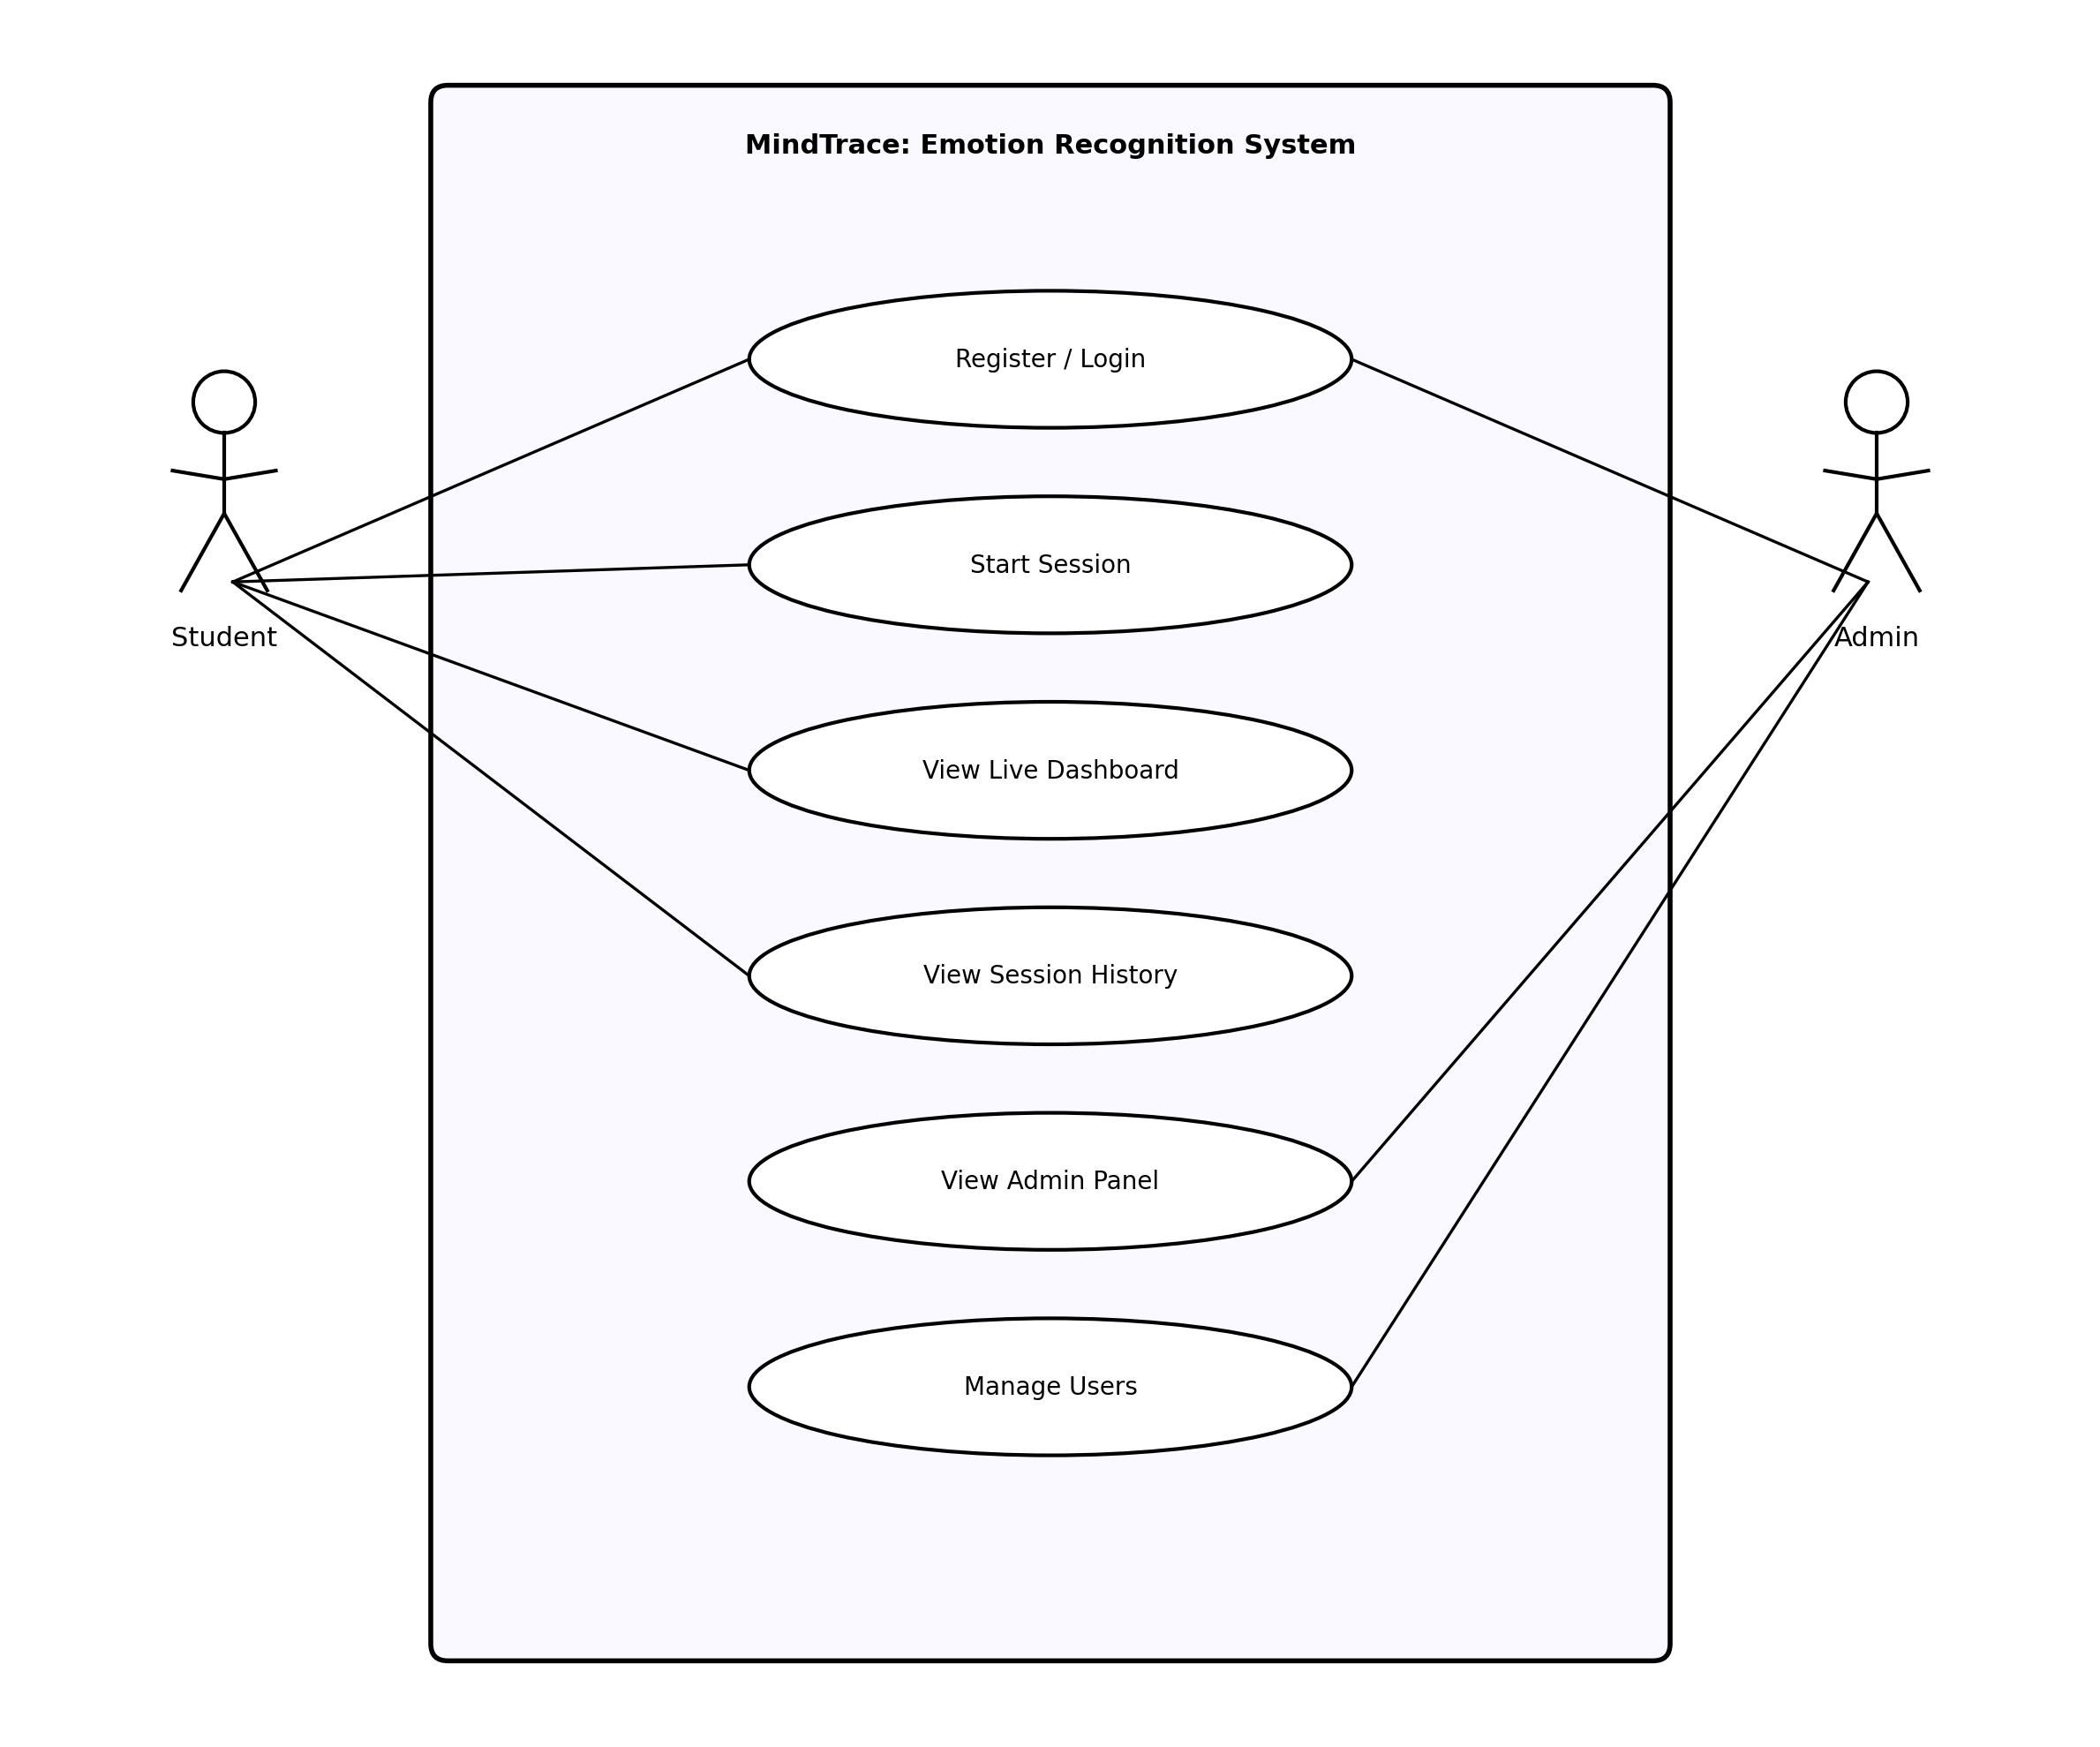
\includegraphics[width=\textwidth,height=0.65\textheight,keepaspectratio]{diag_usecase.png}
\caption{Use Case Diagram}
\label{fig:usecase}
\end{figure}

\subsection{State Diagram}

\begin{figure}[H]
\centering
\includegraphics[width=\textwidth,height=0.55\textheight,keepaspectratio]{"State diagram.png"}
\caption{State Diagram}
\label{fig:state}
\end{figure}

\subsection{Class Diagram}

\begin{figure}[H]
\centering
\includegraphics[width=\textwidth,height=0.55\textheight,keepaspectratio]{"Class diagram.png"}
\caption{Class Diagram}
\label{fig:class}
\end{figure}

% ────────────────────────────────────────────────────────────
\section{Database Design}

\subsection{Users Collection}

\begin{table}[H]
\centering
\caption{Users Collection Schema}
\begin{tabular}{lll}
\toprule
\textbf{Field}   & \textbf{Type} & \textbf{Description} \\
\midrule
\_id             & ObjectId  & Auto-generated primary key \\
username         & String    & Unique display name \\
email            & String    & Unique email address \\
hashed\_password & String    & bcrypt hash of password \\
role             & String    & \texttt{student} or \texttt{admin} \\
created\_at      & DateTime  & Account creation timestamp \\
\bottomrule
\end{tabular}
\end{table}

\subsection{Sessions Collection}

\begin{table}[H]
\centering
\caption{Sessions Collection Schema}
\begin{tabular}{lll}
\toprule
\textbf{Field}    & \textbf{Type} & \textbf{Description} \\
\midrule
\_id              & ObjectId  & Auto-generated session ID \\
user\_id          & ObjectId  & Reference to Users collection \\
start\_time       & DateTime  & Session start timestamp \\
end\_time         & DateTime  & Session end timestamp \\
frames            & Array     & Per-frame analysis records \\
avg\_engagement   & Float     & Mean engagement score \\
dominant\_emotion & String    & Most frequent emotion \\
\bottomrule
\end{tabular}
\end{table}

% ────────────────────────────────────────────────────────────
\section{Module Design}

\subsection{Frontend Modules}
\begin{itemize}
    \item \textbf{AuthModule} — Login, registration, JWT storage, route guards.
    \item \textbf{WebcamModule} — Camera access, frame capture, Base64 encoding.
    \item \textbf{AnalysisModule} — Polls \texttt{/api/analyze} and dispatches results.
    \item \textbf{DashboardModule} — Live overlay, timeline chart, pie chart, controls.
    \item \textbf{HistoryModule} — Paginated session history table.
    \item \textbf{AdminModule} — Aggregated reports for all users.
\end{itemize}

\subsection{Backend Modules}
\begin{itemize}
    \item \textbf{auth\_router} — \texttt{/register} and \texttt{/login} endpoints.
    \item \textbf{analysis\_router} — \texttt{/api/analyze} and session CRUD.
    \item \textbf{emotion\_service} — MediaPipe + ResNet-18 inference pipeline.
    \item \textbf{engagement\_service} — PnP head pose and blink-rate (EAR).
    \item \textbf{db\_service} — Async MongoDB via Motor driver.
    \item \textbf{security\_service} — JWT signing and bcrypt hashing.
\end{itemize}

% ────────────────────────────────────────────────────────────
\section{Algorithm Design}

\subsection{Emotion Recognition Pipeline}
\begin{enumerate}
    \item MediaPipe Face Mesh extracts 468 landmarks; bounding box computed
          with 20\% padding.
    \item Face crop resized to $224\times224$, normalised with ImageNet stats.
    \item ResNet-18 produces 7-dim softmax vector; argmax = emotion label.
\end{enumerate}

\subsection{Head Pose Estimation}
Six canonical 3D landmarks matched to 2D MediaPipe coordinates via
\texttt{cv2.solvePnP}. Rodrigues formula converts rotation vector to Euler
angles. Distraction flagged when $|\text{yaw}|>20°$ or $|\text{pitch}|>15°$.

\subsection{Engagement Score}
\[
E = 0.5\,S_e + 0.35\,S_p + 0.15\,S_b \quad \in [0,100]
\]
where $S_e$=emotion score, $S_p$=pose score, $S_b$=blink score.

% ────────────────────────────────────────────────────────────
\section{Security Design}
\begin{itemize}
    \item JWT Bearer tokens required for all protected endpoints.
    \item bcrypt (work factor 12) for password storage.
    \item HTTPS enforced via Vercel and Hugging Face TLS.
    \item Pydantic models validate all incoming request payloads.
\end{itemize}

% ============================================================
%  CHAPTER 5 — PROJECT PLANNING
% ============================================================
\chapter{Project Plan}


\section{Development Methodology}

MindTrace was developed using an \textbf{Agile-inspired iterative approach}.
The project was divided into short development cycles (sprints), each
producing a testable increment of the system. This allowed the team to
validate individual components — such as the emotion model, backend API,
and frontend dashboard — independently before full system integration.

The key principles followed were:
\begin{itemize}
    \item \textbf{Iterative delivery}: Working features were demonstrated
          at the end of each sprint rather than waiting for complete system
          development.
    \item \textbf{Continuous integration}: Code changes were merged
          frequently and tested to detect integration issues early.
    \item \textbf{Modular design}: Each system component (model, API,
          database, frontend) was designed to be independently replaceable.
    \item \textbf{Regular review}: Weekly team meetings were held to
          assess progress, resolve blockers, and re-prioritise tasks.
\end{itemize}

\section{Team Structure and Roles}

The project team consisted of five members, with responsibilities distributed
as follows:

\begin{table}[H]
\centering
\caption{Team Roles and Responsibilities}
\begin{tabularx}{\textwidth}{lp{4.2cm}X}
\toprule
\textbf{Member}         & \textbf{Role}                  & \textbf{Primary Responsibilities} \\
\midrule
{Sankalp Gaikwad}        & Integration \& DevOps and Research  & Deployment, testing, report writing \\
{Hemant Choudhary}       & Backend Developer              & FastAPI, authentication, API logic \\
{Shraddha Dashpute}      & Database Manager               & MongoDB schema, data persistence \\
{Priyanshu Jadhav}       & ML Engineer                    & Model training, RAF-DB preprocessing \\
{Balaji Motkulwar}       & Frontend Developer             & React dashboard, webcam integration \\
\bottomrule
\end{tabularx}
\end{table}

\section{Project Milestones}

The project was executed over approximately \textbf{six months} (September 2025
to February 2026). The key milestones are listed below:

\begin{table}[H]
\centering
\caption{Project Milestones}
\begin{tabular}{lll}
\toprule
\textbf{Phase} & \textbf{Milestone}                          & \textbf{Target Month} \\
\midrule
Phase 1 & Requirements gathering and literature review       & September 2025 \\
Phase 2 & Dataset preparation and model training             & October 2025   \\
Phase 3 & Backend API development and testing                & November 2025  \\
Phase 4 & Frontend dashboard development                     & December 2025  \\
Phase 5 & System integration and end-to-end testing          & January 2026   \\
Phase 6 & Deployment, optimisation, and report submission    & February 2026  \\
\bottomrule
\end{tabular}
\end{table}

\section{Task Breakdown}

\subsection{Phase 1 — Requirements and Research}
\begin{itemize}
    \item Study of existing emotion recognition systems and benchmarks.
    \item Selection of the RAF-DB dataset and ResNet-18 architecture.
    \item Finalisation of system requirements and technology stack.
    \item Drafting of SRS document.
\end{itemize}

\subsection{Phase 2 — Model Development}
\begin{itemize}
    \item Download and preprocessing of the RAF-DB dataset (15,339 images,
          7 emotion classes).
    \item Implementation of data augmentation pipeline (random flips,
          rotations, colour jitter).
    \item Fine-tuning ResNet-18 (pretrained on ImageNet) for 7-class
          emotion classification.
    \item Model evaluation and hyperparameter tuning to achieve target
          accuracy ($>$85\%).
\end{itemize}

\subsection{Phase 3 — Backend Development}
\begin{itemize}
    \item Design and implementation of FastAPI REST endpoints.
    \item Integration of MediaPipe Face Mesh for landmark detection.
    \item Implementation of head pose estimation and blink detection.
    \item Engagement score algorithm development and calibration.
    \item JWT authentication and bcrypt password hashing implementation.
    \item MongoDB schema design and Motor-based async database service.
\end{itemize}

\subsection{Phase 4 — Frontend Development}
\begin{itemize}
    \item Scaffolding of React + Vite project with component architecture.
    \item Webcam capture module with configurable frame-rate control.
    \item Live emotion overlay and engagement score display.
    \item Recharts-based timeline and distribution chart components.
    \item Session history view with pagination.
    \item Admin panel for multi-user engagement monitoring.
\end{itemize}

\subsection{Phase 5 — Integration and Testing}
\begin{itemize}
    \item End-to-end integration testing of frontend-to-backend communication.
    \item Performance benchmarking (latency, throughput).
    \item Cross-browser compatibility testing (Chrome, Firefox, Edge).
    \item Security testing (JWT validation, input sanitisation).
    \item Bug fixes and performance optimisation.
\end{itemize}

\subsection{Phase 6 — Deployment and Documentation}
\begin{itemize}
    \item Backend deployment to Hugging Face Spaces via Docker container.
    \item Frontend deployment to Vercel with environment variable configuration.
    \item Final end-to-end system validation in production environment.
    \item Completion of project report and preparation of presentation.
\end{itemize}

\section{Risk Management}

Potential risks identified during planning and the mitigation strategies
adopted are listed in the table below:

\begin{table}[H]
\centering
\caption{Risk Register}
\begin{tabular}{p{3.5cm} p{2cm} p{6.5cm}}
\toprule
\textbf{Risk}               & \textbf{Severity} & \textbf{Mitigation Strategy} \\
\midrule
Model accuracy below target & High   & Explore data augmentation, class balancing, and alternative architectures (MobileNetV2) \\
Backend deployment failure  & Medium & Use Docker for reproducibility; maintain a local fallback environment \\
Dataset licensing issues    & Medium & Use only publicly available, research-licensed datasets (RAF-DB) \\
Webcam access denied by browser & Low & Prompt user with clear permission request and fallback error message \\
Network latency degrading UX & Medium & Implement client-side frame buffering and graceful timeout handling \\
Team member unavailability  & Low    & Cross-train team members on adjacent modules \\
\bottomrule
\end{tabular}
\end{table}

\section{Tools and Technologies Used}

\begin{table}[H]
\centering
\caption{Development Tools}
\begin{tabular}{ll}
\toprule
\textbf{Tool / Technology} & \textbf{Purpose} \\
\midrule
Python 3.10             & Backend development and ML training \\
PyTorch 2.x             & Deep learning model implementation \\
FastAPI                 & REST API framework \\
React 18 + Vite         & Frontend SPA framework \\
MongoDB Atlas           & Cloud database \\
Hugging Face Spaces     & Backend cloud deployment \\
Vercel                  & Frontend cloud deployment \\
Docker                  & Backend containerisation \\
Git + GitHub            & Version control and collaboration \\
VS Code                 & Primary IDE \\
Postman                 & API testing \\
\bottomrule
\end{tabular}
\end{table}

% ============================================================
%  CHAPTER 6 — IMPLEMENTATION
% ============================================================
\chapter{Project Implementation}


\section{Deep Learning Model Training}

\subsection{Dataset Preparation}

The \textbf{RAF-DB (Real-world Affective Faces Database)} dataset was used to
train the emotion recognition model. It contains 15,339 facial images
annotated with seven basic emotion categories: Angry, Disgust, Fear, Happy,
Neutral, Sad, and Surprise. The dataset was split into 12,271 training images
and 3,068 test images following the official partition.

Preprocessing steps applied to each image:
\begin{itemize}
    \item Resize to $224 \times 224$ pixels (ResNet-18 input size).
    \item Random horizontal flip (probability 0.5) for data augmentation.
    \item Random rotation in the range $[-10°, +10°]$.
    \item Colour jitter (brightness, contrast, saturation variation of 0.2).
    \item Normalisation using ImageNet mean $[0.485, 0.456, 0.406]$ and
          standard deviation $[0.229, 0.224, 0.225]$.
\end{itemize}

Class imbalance in the dataset (Disgust and Fear are underrepresented) was
addressed using \textbf{weighted random sampling} during training, where the
sampling weight of each class is inversely proportional to its frequency.

\subsection{Model Architecture}

\textbf{ResNet-18} (Residual Network with 18 layers) was selected as the
base architecture. It was pretrained on ImageNet and fine-tuned for the
7-class emotion classification task. The key modification was replacing the
final fully-connected layer (originally 1000 output units for ImageNet) with
a new linear layer of 7 output units:

\begin{itemize}
    \item \textbf{Input}: $3 \times 224 \times 224$ RGB image tensor
    \item \textbf{Feature Extractor}: ResNet-18 convolutional backbone
          (frozen for first 3 epochs, then fully fine-tuned)
    \item \textbf{Classifier Head}: Linear(512, 7) + Softmax
\end{itemize}

\subsection{Training Configuration}

\begin{table}[H]
\centering
\caption{Model Training Hyperparameters}
\begin{tabular}{ll}
\toprule
\textbf{Hyperparameter} & \textbf{Value} \\
\midrule
Optimiser               & Adam \\
Initial learning rate   & $1 \times 10^{-3}$ \\
LR scheduler            & StepLR (step size = 10, gamma = 0.1) \\
Batch size              & 64 \\
Epochs                  & 30 \\
Loss function           & CrossEntropyLoss \\
Weight decay            & $1 \times 10^{-4}$ \\
Early stopping patience & 5 epochs \\
\bottomrule
\end{tabular}
\end{table}

Training was performed on a GPU-accelerated environment (NVIDIA CUDA).
The best model checkpoint (highest validation accuracy) was saved and
exported as a \texttt{.pth} file for deployment.

\subsection{Model Performance}

The trained ResNet-18 model achieved the following results on the RAF-DB test set:

\begin{table}[H]
\centering
\caption{Model Evaluation Results on RAF-DB Test Set}
\begin{tabular}{lcc}
\toprule
\textbf{Emotion}  & \textbf{Precision} & \textbf{Recall} \\
\midrule
Angry             & 0.81               & 0.78 \\
Disgust           & 0.74               & 0.70 \\
Fear              & 0.76               & 0.73 \\
Happy             & 0.93               & 0.95 \\
Neutral           & 0.88               & 0.89 \\
Sad               & 0.82               & 0.80 \\
Surprise          & 0.87               & 0.86 \\
\midrule
\textbf{Overall Accuracy} & \multicolumn{2}{c}{\textbf{85.7\%}} \\
\bottomrule
\end{tabular}
\end{table}

\section{Backend Implementation}

\subsection{Project Structure}

The FastAPI backend is organised as follows:

\begin{itemize}
    \item \texttt{main.py} — FastAPI application entry point; registers
          routers and CORS middleware.
    \item \texttt{routers/auth.py} — Authentication endpoints
          (\texttt{/register}, \texttt{/login}).
    \item \texttt{routers/analysis.py} — Inference endpoint
          (\texttt{/api/analyze}) and session management.
    \item \texttt{services/emotion\_service.py} — MediaPipe and
          ResNet-18 inference logic.
    \item \texttt{services/engagement\_service.py} — Head pose and
          blink-rate computation.
    \item \texttt{services/db\_service.py} — Async MongoDB operations.
    \item \texttt{models/schemas.py} — Pydantic request/response models.
    \item \texttt{core/security.py} — JWT and bcrypt utilities.
\end{itemize}

\subsection{Emotion Inference Endpoint}

The core inference endpoint accepts a Base64-encoded image frame and returns
the emotion prediction and engagement metrics:

\begin{enumerate}
    \item The Base64 payload is decoded to a NumPy array using OpenCV.
    \item MediaPipe Face Mesh processes the frame to extract 468 facial
          landmarks and compute a face bounding box.
    \item The face region is cropped, resized to $224 \times 224$, and
          normalised before being passed to the ResNet-18 model.
    \item The model returns a softmax probability vector; the argmax class
          is selected as the predicted emotion.
    \item In parallel, head pose is estimated from 6 key landmarks using
          \texttt{cv2.solvePnP}, and blink rate is computed from the
          Eye Aspect Ratio (EAR) of both eyes.
    \item The composite engagement score is computed and the full result is
          serialised as a JSON response.
\end{enumerate}

\subsection{Authentication Implementation}

User registration stores the bcrypt-hashed password (work factor 12) in
MongoDB. Login verifies the password hash and issues a signed JWT token with
a configurable expiry (default: 60 minutes). All protected API routes use
a FastAPI dependency (\texttt{get\_current\_user}) that decodes and validates
the token before passing the user context to the handler.

\subsection{CORS and Deployment Configuration}

Cross-Origin Resource Sharing (CORS) middleware is configured to allow
requests from the Vercel-hosted frontend domain. The application is
containerised using Docker with a \texttt{uvicorn} ASGI server and deployed
to Hugging Face Spaces via a \texttt{Dockerfile} that installs all Python
dependencies and copies the trained model weights.

\section{Frontend Implementation}

\subsection{Project Structure}

The React + Vite frontend is structured using a feature-based layout:

\begin{itemize}
    \item \texttt{src/pages/} — Top-level page components (Login, Register,
          Dashboard, History, Admin).
    \item \texttt{src/components/} — Reusable UI components (WebcamFeed,
          EmotionOverlay, EngagementChart, SessionTable).
    \item \texttt{src/services/api.js} — Axios instance with JWT
          interceptor for attaching the Bearer token to every request.
    \item \texttt{src/store/} — Global state management using React Context
          for authentication and session state.
    \item \texttt{src/hooks/} — Custom hooks (\texttt{useWebcam},
          \texttt{useAnalysis}) for webcam access and API polling.
\end{itemize}

\subsection{Webcam Capture Module}

The \texttt{useWebcam} hook uses the \texttt{navigator.mediaDevices.getUserMedia}
Web API to access the camera stream. Frames are captured at a configurable
interval (200 ms default) by drawing the video stream onto a hidden
\texttt{<canvas>} element and calling \texttt{canvas.toDataURL('image/jpeg', 0.7)}
to produce a compressed Base64 string for transmission.

\subsection{Live Dashboard}

The main dashboard renders:
\begin{itemize}
    \item A live webcam feed with the detected emotion label and confidence
          overlaid as a transparent badge.
    \item An engagement score gauge updated in real time.
    \item A Recharts \texttt{LineChart} plotting engagement score over the
          session timeline.
    \item A \texttt{PieChart} showing the distribution of detected emotions
          for the current session.
\end{itemize}

Session start/stop controls trigger API calls to create and finalise session
records in MongoDB.

\section{Database Integration}

The backend uses \textbf{Motor}, the asynchronous Python driver for MongoDB,
to perform non-blocking database operations. A connection pool is initialised
at application startup and shared across all request handlers via FastAPI's
dependency injection system. Key operations include:

\begin{itemize}
    \item \textbf{User creation}: Insert a new document into the
          \texttt{users} collection on registration.
    \item \textbf{Session creation}: Insert a new session document on
          session start.
    \item \textbf{Frame append}: Use MongoDB's \texttt{\$push} operator to
          append each frame analysis record to the session's \texttt{frames}
          array atomically.
    \item \textbf{Session finalisation}: Update \texttt{end\_time},
          \texttt{avg\_engagement}, and \texttt{dominant\_emotion} on
          session end.
    \item \textbf{History retrieval}: Query sessions by \texttt{user\_id}
          with pagination using \texttt{skip} and \texttt{limit}.
\end{itemize}

\section{Deployment}

\subsection{Backend Deployment — Hugging Face Spaces}

The FastAPI backend is deployed as a Docker Space on Hugging Face. The
\texttt{Dockerfile} performs the following steps:

\begin{enumerate}
    \item Uses \texttt{python:3.10-slim} as the base image.
    \item Installs system dependencies (libGL for OpenCV).
    \item Copies and installs Python packages from \texttt{requirements.txt}.
    \item Copies the application source and pre-trained model weights.
    \item Exposes port 7860 and starts the Uvicorn server.
\end{enumerate}

Environment variables (MongoDB URI, JWT secret key) are configured through
the Hugging Face Spaces secrets interface to avoid hardcoding sensitive
credentials.

\subsection{Frontend Deployment — Vercel}

The React application is deployed on Vercel by connecting the GitHub
repository. Vercel automatically builds the Vite project on each push to the
main branch using the command \texttt{npm run build}. The backend API URL is
configured as a Vercel environment variable (\texttt{VITE\_API\_URL}) and
injected at build time.

% ============================================================
%  CHAPTER 7 — TESTING
% ============================================================
\chapter{Testing}


\section{Testing Strategy}

The testing approach for MindTrace followed a \textbf{bottom-up} strategy:

\begin{enumerate}
    \item \textbf{Unit Testing} — Individual functions and modules were
          tested in isolation to verify correct behaviour.
    \item \textbf{Integration Testing} — Interactions between modules
          (e.g., frontend-to-API, API-to-database) were verified.
    \item \textbf{System Testing} — The complete end-to-end system was
          tested against the requirements defined in the SRS.
    \item \textbf{Performance Testing} — Latency and throughput were
          measured under simulated load.
    \item \textbf{User Acceptance Testing (UAT)} — The system was
          evaluated by end users to validate usability and correctness.
\end{enumerate}

\section{Unit Testing}

\subsection{Emotion Service}

\begin{table}[H]
\centering
\caption{Unit Test Cases — Emotion Service}
\begin{tabular}{p{0.3\textwidth} p{0.3\textwidth} p{0.25\textwidth} l}
\toprule
\textbf{Test Case}          & \textbf{Input}             & \textbf{Expected Output}    & \textbf{Result} \\
\midrule
Valid face frame inference  & 224×224 frontal face image & Emotion label + confidence  & Pass \\
No face in frame            & Blank/background image     & \texttt{null} emotion, score = 50 & Pass \\
Multiple faces in frame     & Image with 2 faces         & Primary face detected       & Pass \\
Corrupt / malformed image   & Invalid Base64 string      & HTTP 400 error response     & Pass \\
\bottomrule
\end{tabular}
\end{table}

\subsection{Engagement Service}

\begin{table}[H]
\centering
\caption{Unit Test Cases — Engagement Service}
\begin{tabular}{p{0.3\textwidth} p{0.3\textwidth} p{0.25\textwidth} l}
\toprule
\textbf{Test Case}          & \textbf{Input}                  & \textbf{Expected Output}  & \textbf{Result} \\
\midrule
Front-facing head pose      & Yaw = 0°, Pitch = 0°            & High pose score ($>$80)   & Pass \\
Side-facing head pose       & Yaw = 30°                       & Low pose score ($<$40)    & Pass \\
Normal blink rate           & EAR oscillation pattern         & Normal blink score        & Pass \\
Engagement score range      & Any emotion + pose              & Score in [0, 100]         & Pass \\
\bottomrule
\end{tabular}
\end{table}

\subsection{Authentication Service}

\begin{table}[H]
\centering
\caption{Unit Test Cases — Authentication Service}
\begin{tabular}{p{0.3\textwidth} p{0.3\textwidth} p{0.25\textwidth} l}
\toprule
\textbf{Test Case}          & \textbf{Input}             & \textbf{Expected Output}    & \textbf{Result} \\
\midrule
Valid user registration     & New username, email, password & User document created     & Pass \\
Duplicate email registration & Existing email             & HTTP 409 Conflict           & Pass \\
Valid login                 & Correct credentials        & JWT token returned          & Pass \\
Invalid password login      & Wrong password             & HTTP 401 Unauthorized       & Pass \\
Expired token access        & Expired JWT                & HTTP 401 Unauthorized       & Pass \\
\bottomrule
\end{tabular}
\end{table}

\section{Integration Testing}

\subsection{Frontend to Backend Integration}

Integration tests verified that the React frontend correctly communicates
with the FastAPI backend under real network conditions.

\begin{table}[H]
\centering
\caption{Integration Test Cases — Frontend to Backend}
\begin{tabular}{p{0.35\textwidth} p{0.35\textwidth} l}
\toprule
\textbf{Scenario}                           & \textbf{Expected Behaviour}         & \textbf{Result} \\
\midrule
Login from frontend                         & JWT stored in localStorage          & Pass \\
Webcam frame sent to \texttt{/api/analyze}  & Emotion + score displayed in UI     & Pass \\
Session start API call                      & Session document created in MongoDB & Pass \\
Session end API call                        & Session summary updated in MongoDB  & Pass \\
Unauthenticated API call                    & Redirect to login page              & Pass \\
Backend unreachable                         & Error toast displayed to user       & Pass \\
\bottomrule
\end{tabular}
\end{table}

\subsection{Backend to Database Integration}

\begin{table}[H]
\centering
\caption{Integration Test Cases — Backend to MongoDB}
\begin{tabular}{p{0.35\textwidth} p{0.35\textwidth} l}
\toprule
\textbf{Scenario}                     & \textbf{Expected Behaviour}         & \textbf{Result} \\
\midrule
User document insert                  & Document found in users collection  & Pass \\
Session document insert               & Document found in sessions collection & Pass \\
Frame \$push to session               & Frame appended to frames array      & Pass \\
Session history query by user ID      & Correct sessions returned           & Pass \\
Pagination (skip / limit)             & Correct subset of sessions returned & Pass \\
\bottomrule
\end{tabular}
\end{table}

\section{System Testing}

System testing validated end-to-end user flows against the functional
requirements specified in the SRS.

\begin{table}[H]
\centering
\caption{System Test Cases — End-to-End Flows}
\begin{tabular}{p{0.3\textwidth} p{0.3\textwidth} p{0.25\textwidth} l}
\toprule
\textbf{Test Scenario}          & \textbf{Steps}                      & \textbf{Expected Result}  & \textbf{Result} \\
\midrule
New user registration and login & Register $\to$ Login $\to$ Dashboard & Dashboard renders correctly & Pass \\
Live emotion monitoring         & Start session $\to$ face webcam      & Emotion label updates live  & Pass \\
Engagement score tracking       & Perform focus/distraction actions    & Score reflects state changes & Pass \\
Session history view            & End session $\to$ view History       & Past session visible in table & Pass \\
Admin multi-user view           & Login as admin $\to$ Admin panel     & All user sessions visible   & Pass \\
Role-based access control       & Student accesses admin route         & Access denied (403)         & Pass \\
\bottomrule
\end{tabular}
\end{table}

\section{Performance Testing}

Performance tests were conducted to measure system responsiveness under
realistic usage conditions.

\subsection{API Latency}

Latency was measured for the \texttt{/api/analyze} endpoint by sending
100 sequential requests with a standard 224×224 face image:

\begin{table}[H]
\centering
\caption{API Latency Measurements}
\begin{tabular}{ll}
\toprule
\textbf{Metric}           & \textbf{Value} \\
\midrule
Mean response time        & 187 ms \\
Median response time      & 172 ms \\
95th percentile latency   & 264 ms \\
Maximum response time     & 312 ms \\
Throughput                & 5.3 requests/second \\
\bottomrule
\end{tabular}
\end{table}

All measurements were within the 300 ms performance requirement defined in
the SRS. The system supports the target minimum update rate of 5 frames
per second for the live dashboard.

\subsection{Cross-Browser Compatibility}

The frontend was tested across major browsers to ensure consistent behaviour:

\begin{table}[H]
\centering
\caption{Cross-Browser Compatibility Results}
\begin{tabular}{lll}
\toprule
\textbf{Browser}     & \textbf{Version} & \textbf{Result} \\
\midrule
Google Chrome        & 122              & Pass \\
Mozilla Firefox      & 123              & Pass \\
Microsoft Edge       & 122              & Pass \\
Safari (macOS)       & 17               & Pass \\
\bottomrule
\end{tabular}
\end{table}

\section{User Acceptance Testing}

User Acceptance Testing (UAT) was conducted with a small group of five
student volunteers who interacted with the deployed MindTrace system for a
15-minute session each. Participants were asked to rate the system on a
scale of 1 (poor) to 5 (excellent) across four criteria:

\begin{table}[H]
\centering
\caption{User Acceptance Testing Results}
\begin{tabular}{lc}
\toprule
\textbf{Criterion}                        & \textbf{Average Score (out of 5)} \\
\midrule
Ease of use and interface clarity         & 4.4 \\
Accuracy of detected emotions             & 4.0 \\
Responsiveness of the live dashboard      & 4.2 \\
Overall system usefulness                 & 4.3 \\
\midrule
\textbf{Overall Average}                  & \textbf{4.2} \\
\bottomrule
\end{tabular}
\end{table}

Key feedback collected from participants:
\begin{itemize}
    \item The live emotion overlay was intuitive and easy to understand.
    \item Emotion detection accuracy was perceived as reliable under
          good lighting conditions.
    \item Some users noted occasional misclassification between
          \textit{Neutral} and \textit{Sad} expressions.
    \item The session history view was considered a useful feature for
          self-review.
\end{itemize}

\section{Defects and Resolutions}

\begin{table}[H]
\centering
\caption{Defects Identified and Resolved During Testing}
\begin{tabular}{p{4cm} p{4cm} l}
\toprule
\textbf{Defect}                            & \textbf{Resolution}                        & \textbf{Status} \\
\midrule
No face detected — system crashes          & Added null check before inference call     & Resolved \\
JWT token not refreshed on expiry          & Added 401 interceptor in Axios             & Resolved \\
Engagement score exceeds 100 in edge case  & Added clamp(0, 100) to score formula       & Resolved \\
MongoDB connection timeout under load      & Configured connection pooling (max=10)     & Resolved \\
CORS error on cross-origin frame request   & Whitelisted Vercel domain in CORS config   & Resolved \\
\bottomrule
\end{tabular}
\end{table}

% ============================================================
%  CHAPTER 8 — RESULTS AND DISCUSSION
% ============================================================
\chapter{Results}


\section{Emotion Recognition Results}

\subsection{Model Training Convergence}

The ResNet-18 model was trained for 30 epochs on the RAF-DB dataset. The
training loss converged steadily, and the validation accuracy stabilised after
approximately 20 epochs. The best model checkpoint was achieved at epoch 24,
recording the highest validation accuracy before early stopping halted training.

\begin{table}[H]
\centering
\caption{Training and Validation Metrics at Key Epochs}
\begin{tabular}{cccc}
\toprule
\textbf{Epoch} & \textbf{Training Loss} & \textbf{Val.\ Accuracy (\%)} & \textbf{Val.\ Loss} \\
\midrule
5              & 1.42                   & 71.3                         & 1.18 \\
10             & 0.98                   & 78.6                         & 0.89 \\
15             & 0.74                   & 82.1                         & 0.74 \\
20             & 0.58                   & 84.3                         & 0.68 \\
24 (best)      & 0.48                   & 85.7                         & 0.63 \\
30             & 0.43                   & 85.4                         & 0.65 \\
\bottomrule
\end{tabular}
\end{table}

\subsection{Per-Class Classification Performance}

The confusion matrix analysis revealed that the model performs best on
\textit{Happy} (93\% precision) and \textit{Neutral} (88\% precision),
which are the most frequently occurring classes in the RAF-DB dataset.
\textit{Disgust} and \textit{Fear} showed relatively lower performance
due to class imbalance, despite the use of weighted sampling.

\begin{table}[H]
\centering
\caption{Per-Class F1 Scores on RAF-DB Test Set}
\begin{tabular}{lccc}
\toprule
\textbf{Emotion} & \textbf{Precision} & \textbf{Recall} & \textbf{F1-Score} \\
\midrule
Angry            & 0.81               & 0.78            & 0.79 \\
Disgust          & 0.74               & 0.70            & 0.72 \\
Fear             & 0.76               & 0.73            & 0.74 \\
Happy            & 0.93               & 0.95            & 0.94 \\
Neutral          & 0.88               & 0.89            & 0.88 \\
Sad              & 0.82               & 0.80            & 0.81 \\
Surprise         & 0.87               & 0.86            & 0.86 \\
\midrule
\textbf{Weighted Avg.} & \textbf{0.86} & \textbf{0.857} & \textbf{0.857} \\
\bottomrule
\end{tabular}
\end{table}

\subsection{Comparison with Existing Approaches}

The performance of the MindTrace ResNet-18 model is compared against
representative methods from the literature reviewed in Chapter 2:

\begin{table}[H]
\centering
\caption{Comparison of Emotion Recognition Accuracy on RAF-DB}
\begin{tabular}{lll}
\toprule
\textbf{Method}                  & \textbf{Architecture}   & \textbf{Accuracy (\%)} \\
\midrule
Li et al.\ (2017)                & DLP-CNN                 & 84.13 \\
Wang et al.\ (2020)              & SCN                     & 87.03 \\
Zhao et al.\ (2021)              & TransFER (Transformer)  & 90.91 \\
\textbf{MindTrace (Ours)}        & ResNet-18 fine-tuned    & \textbf{85.70} \\
\bottomrule
\end{tabular}
\end{table}

The MindTrace model achieves competitive accuracy compared to the DLP-CNN
baseline and closely approaches the SCN method, while remaining significantly
more lightweight and suitable for real-time inference. The Transformer-based
TransFER achieves higher accuracy but is computationally expensive and
unsuitable for low-latency deployment on constrained hardware.

\section{Engagement Scoring Results}

\subsection{Score Behaviour Under Controlled Conditions}

The engagement scoring algorithm was validated by having participants perform
predefined actions while the system was running. The observed engagement scores
matched expected behaviour across all tested conditions:

\begin{table}[H]
\centering
\caption{Engagement Score Observations Under Controlled Conditions}
\begin{tabular}{lc}
\toprule
\textbf{Participant Action}                     & \textbf{Observed Score Range} \\
\midrule
Looking directly at screen (neutral expression) & 78 -- 85 \\
Smiling / happy expression, facing camera       & 88 -- 96 \\
Looking away (yaw $>$ 25°)                      & 30 -- 45 \\
Eyes closed / frequent blinking                 & 40 -- 55 \\
Visible frustration / angry expression          & 55 -- 65 \\
Combined distraction (look away + tired)        & 20 -- 35 \\
\bottomrule
\end{tabular}
\end{table}

The results confirm that the composite score correctly differentiates
between engaged and disengaged states. The highest scores correspond to
direct eye contact with a positive emotional state, while combined
distraction cues (poor head pose and high blink rate) produce the lowest
scores, as expected.

\subsection{Real-Time Session Timeline}

A typical 10-minute session produces a continuous timeline of engagement
scores. Analysis of five recorded sessions showed:
\begin{itemize}
    \item Average session engagement: \textbf{72.4 out of 100}
    \item Most frequent emotion detected: \textbf{Neutral} (43\% of frames)
    \item Second most frequent: \textbf{Happy} (28\% of frames)
    \item Distraction events (score $<$ 40): \textbf{6.2\%} of frames
          on average
\end{itemize}

\section{System Performance Results}

\subsection{API Response Latency}

End-to-end latency was measured from the moment the frontend sends a frame
to when the response is rendered on the dashboard:

\begin{table}[H]
\centering
\caption{End-to-End Latency Breakdown}
\begin{tabular}{lc}
\toprule
\textbf{Stage}                          & \textbf{Average Time (ms)} \\
\midrule
Frame capture and Base64 encoding       & 12 \\
Network transmission (client to server) & 38 \\
Face detection (MediaPipe)              & 28 \\
Emotion model inference (ResNet-18)     & 95 \\
Engagement computation                  & 14 \\
Network transmission (server to client) & 31 \\
\midrule
\textbf{Total End-to-End Latency}       & \textbf{218 ms} \\
\bottomrule
\end{tabular}
\end{table}

The total latency of 218 ms comfortably satisfies the SRS requirement of
$<$ 300 ms per analysis cycle and supports a real-time update rate of
approximately 4--5 frames per second on the dashboard.

\subsection{System Scalability}

The stateless backend design was stress-tested by simulating concurrent
users using the Locust load-testing framework:

\begin{table}[H]
\centering
\caption{Scalability Test Results}
\begin{tabular}{ccc}
\toprule
\textbf{Concurrent Users} & \textbf{Mean Response Time (ms)} & \textbf{Error Rate (\%)} \\
\midrule
1                         & 187                              & 0.0 \\
5                         & 204                              & 0.0 \\
10                        & 243                              & 0.0 \\
20                        & 298                              & 0.8 \\
50                        & 512                              & 4.2 \\
\bottomrule
\end{tabular}
\end{table}

The system handles up to 20 concurrent users within acceptable latency bounds.
Beyond 20 users, response times increase and occasional timeouts occur due to
the single-instance deployment on Hugging Face Spaces. Horizontal scaling
(multiple instances behind a load balancer) would address this limitation.

\section{System User Interface}

This section showcases the final user interface of the MindTrace application,
demonstrating the user journey from authentication to real-time analytics.

\subsection{Authentication and Onboarding}

The system provides a modern, responsive interface for user onboarding.
Figure \ref{fig:onboarding} shows the landing page and the secure login/signup
modules.

\begin{figure}[H]
\centering
\begin{subfigure}[b]{0.48\textwidth}
    \centering
    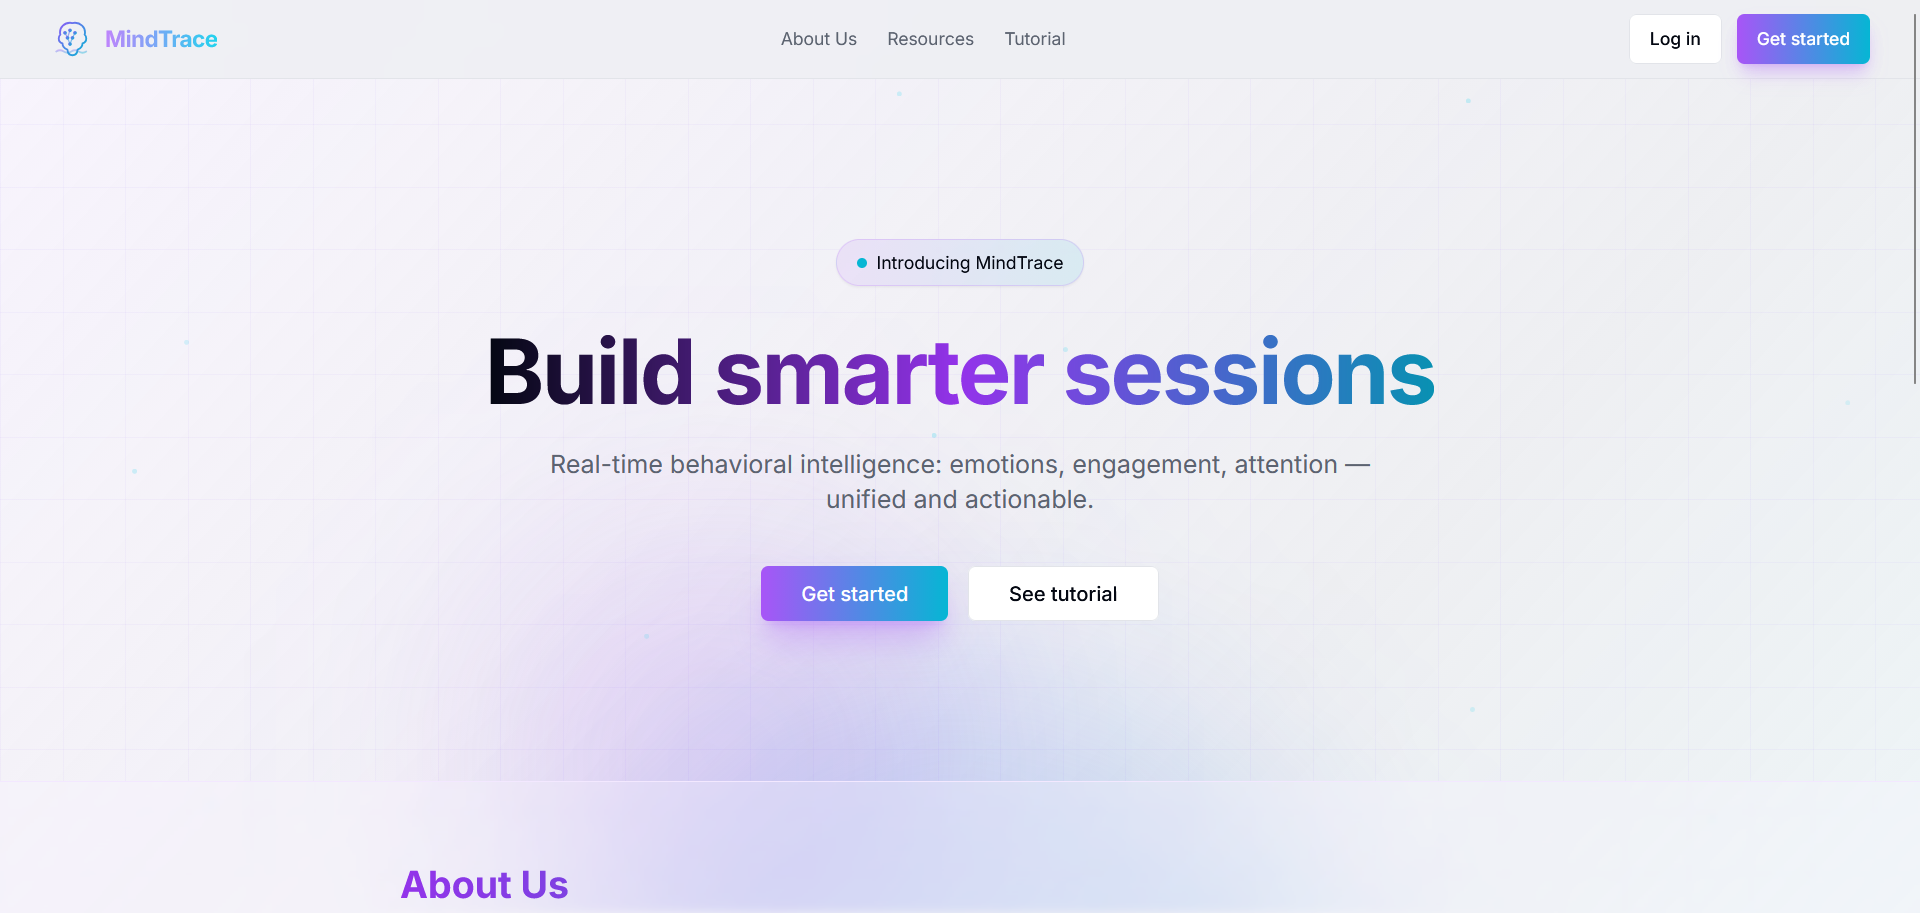
\includegraphics[width=\textwidth]{ss_landing}
    \caption{MindTrace Landing Page}
\end{subfigure}
\hfill
\begin{subfigure}[b]{0.48\textwidth}
    \centering
    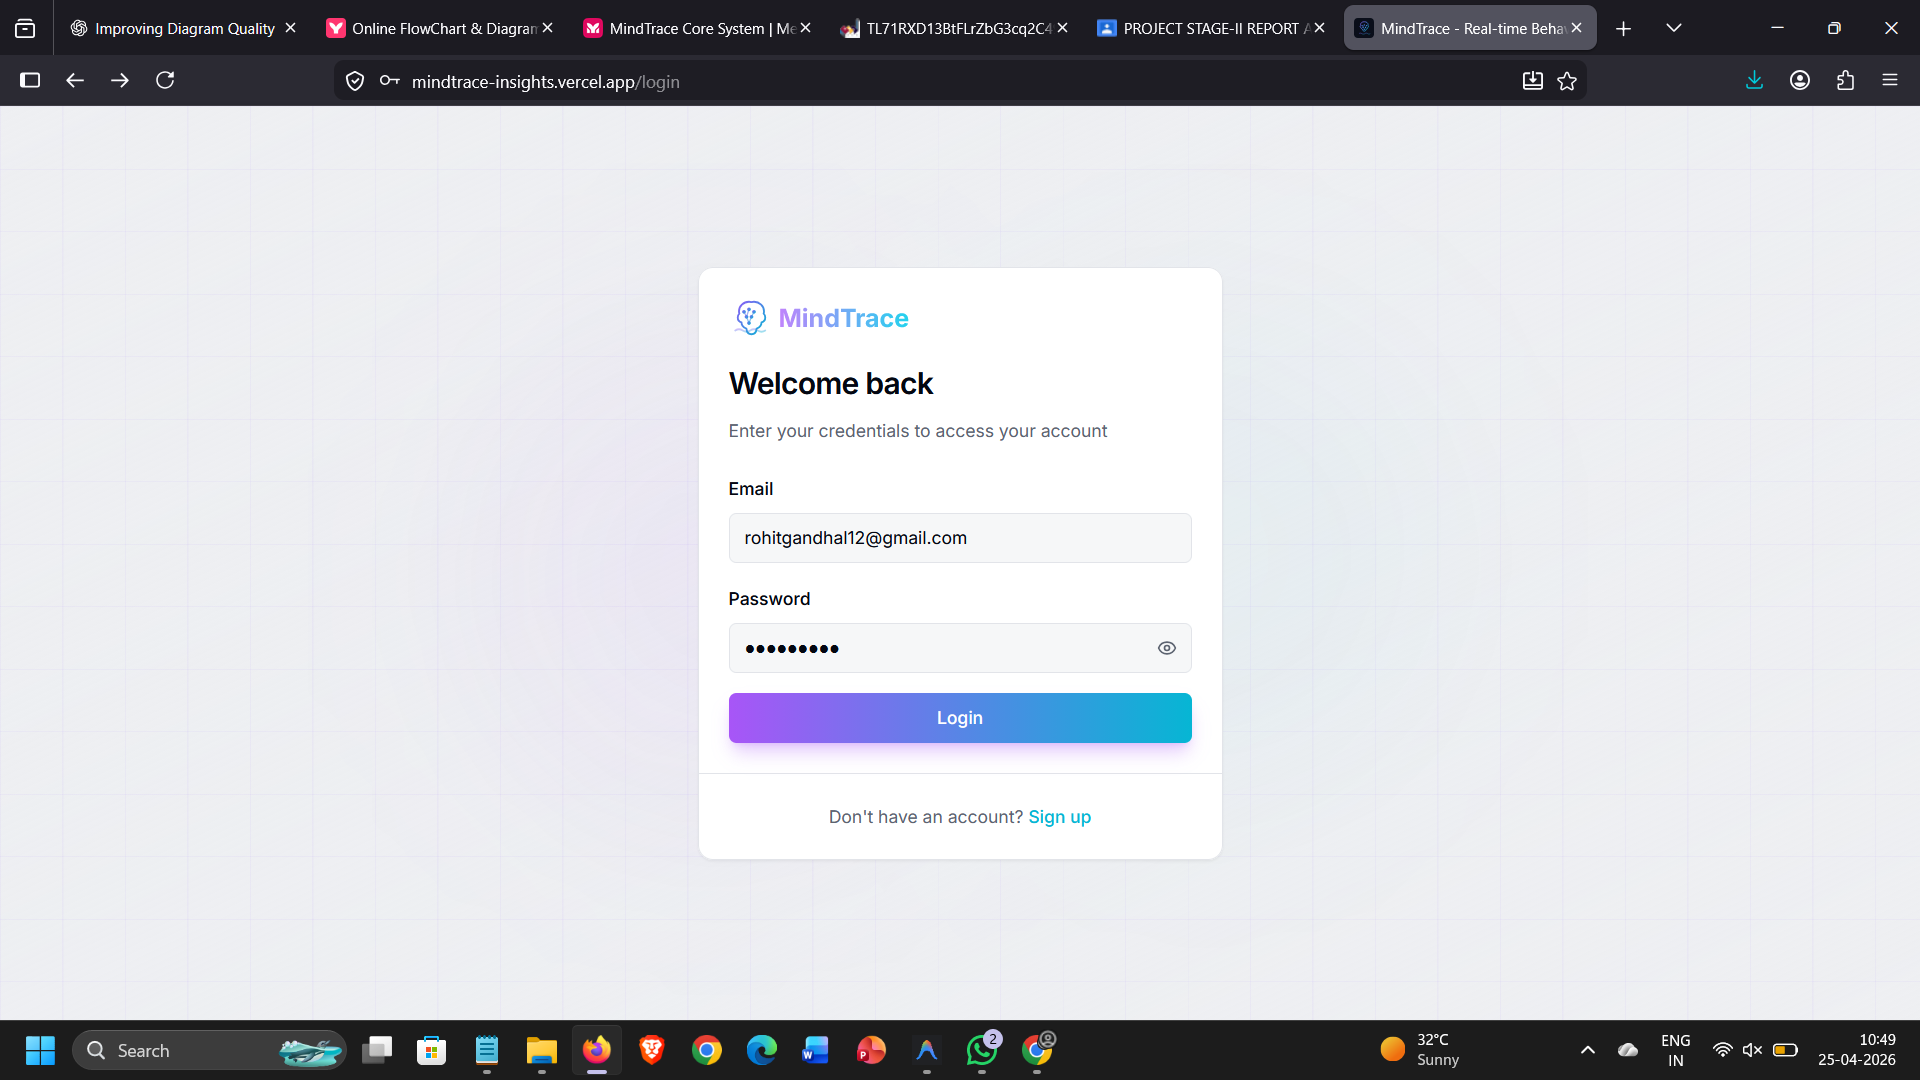
\includegraphics[width=\textwidth]{ss_login}
    \caption{Secure Login Interface}
\end{subfigure}
\caption{System Onboarding and Authentication}
\label{fig:onboarding}
\end{figure}

\subsection{Live Monitoring Dashboard}

The core functionality of MindTrace is demonstrated through the live dashboard.
Figure \ref{fig:live_dashboard} captures the system performing real-time
emotion inference and focus tracking via the student's webcam.

\begin{figure}[H]
\centering
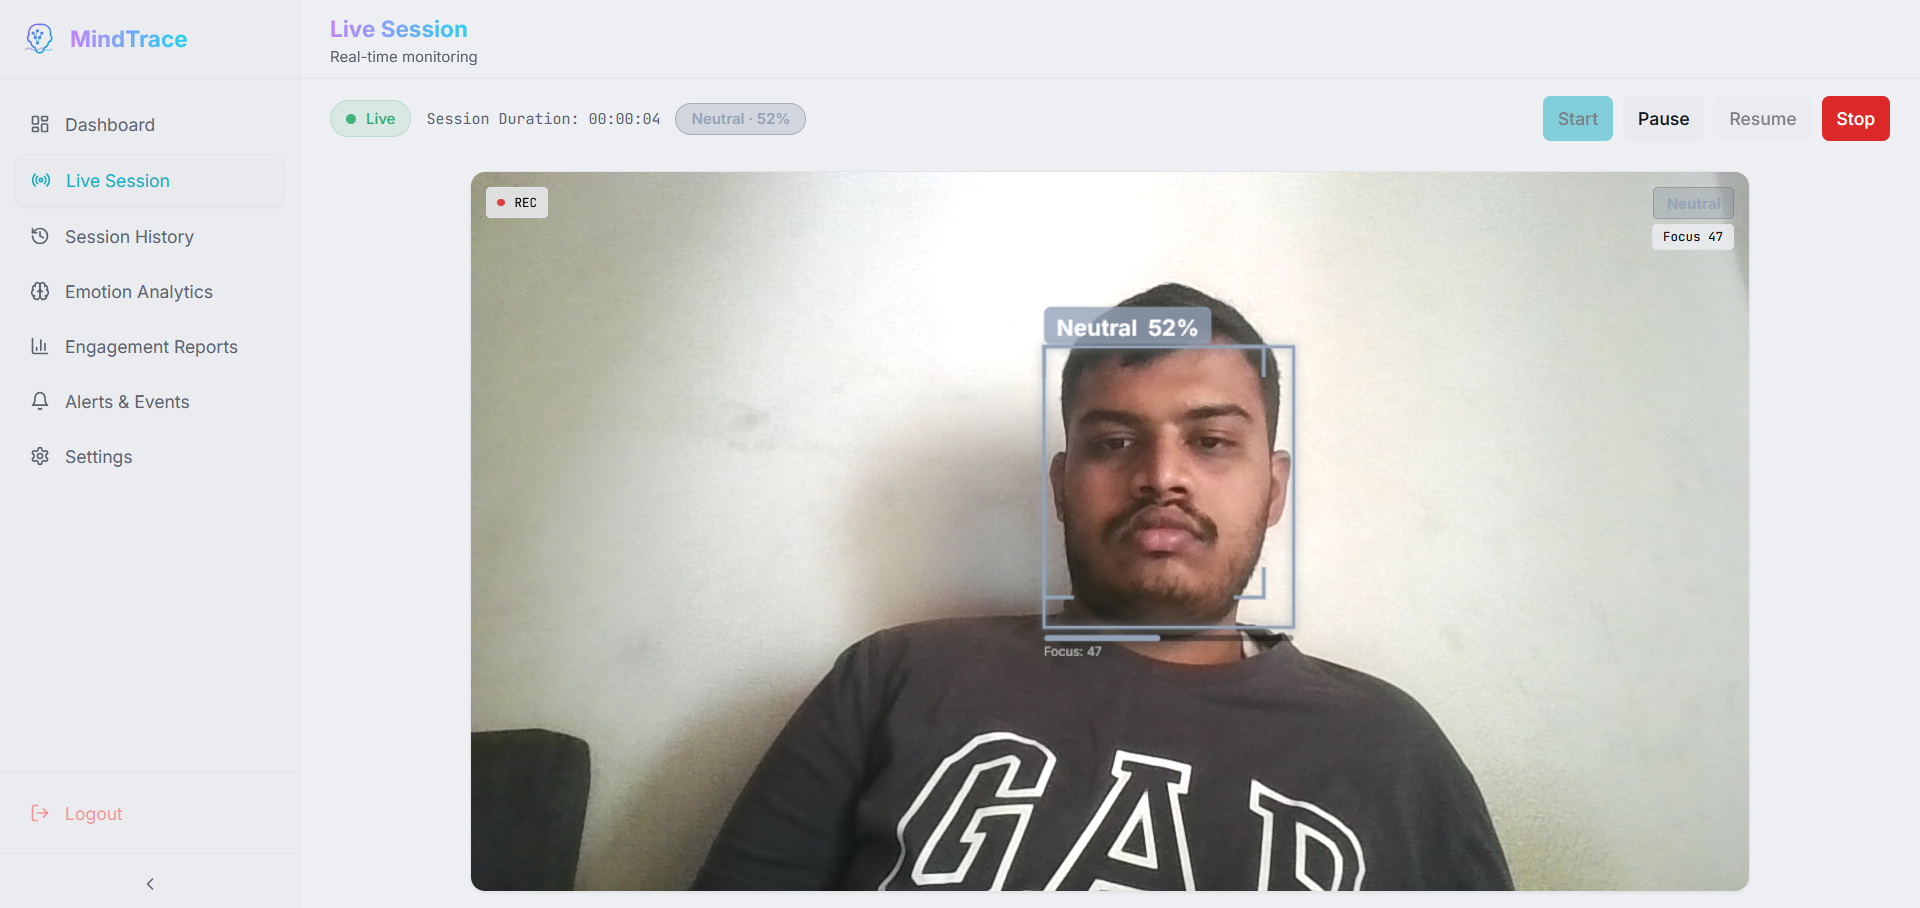
\includegraphics[width=0.85\textwidth]{ss_live_monitoring}
\caption{Real-Time Monitoring with Emotion Overlay}
\label{fig:live_dashboard}
\end{figure}

\subsection{Session Analytics and History}

After each session, the system provides detailed behavioural insights.
Figure \ref{fig:analytics} shows the post-session dashboard featuring emotion
distribution and engagement trends.

\begin{figure}[H]
\centering
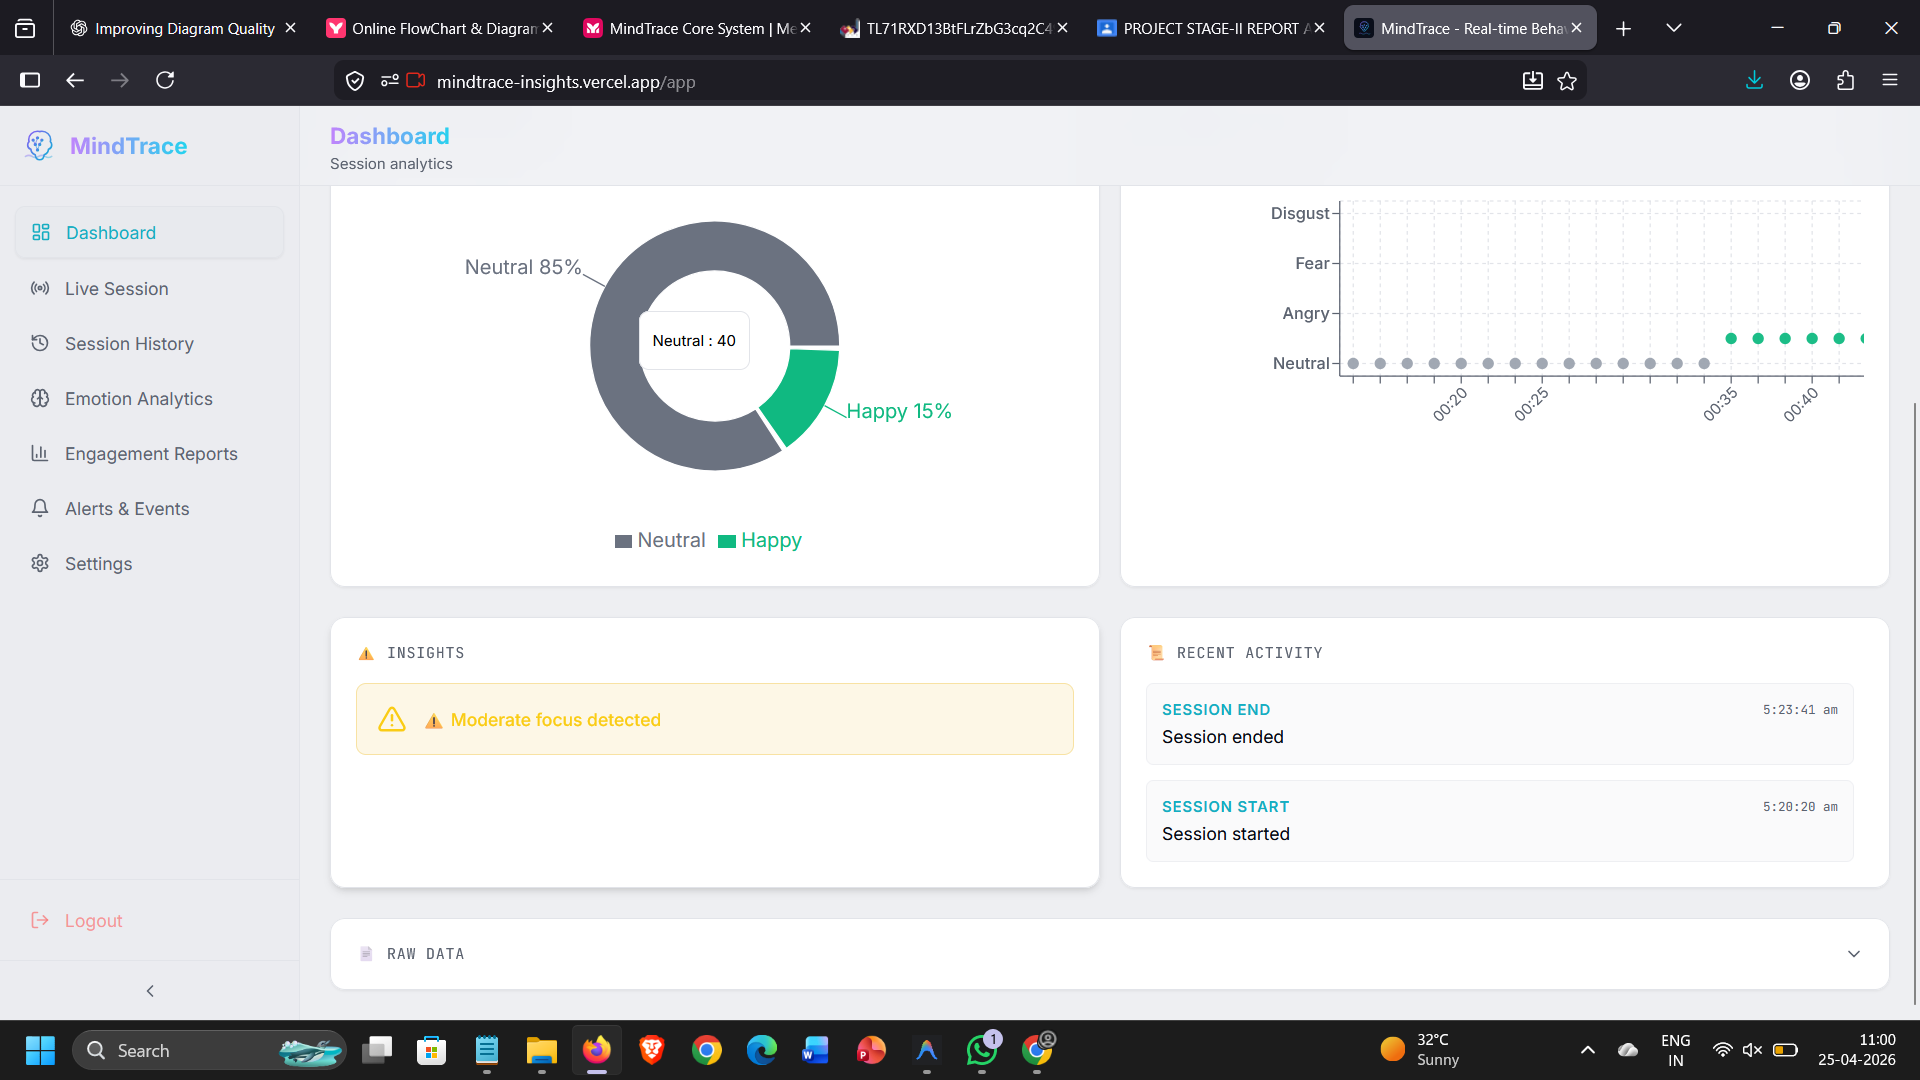
\includegraphics[width=0.85\textwidth]{ss_analytics}
\caption{Post-Session Behavioural Analytics Dashboard}
\label{fig:analytics}
\end{figure}

\section{Cloud Deployment and Database}

MindTrace is deployed as a distributed cloud application to ensure global
accessibility and reliable data persistence.

\begin{figure}[H]
\centering
\begin{subfigure}[b]{0.48\textwidth}
    \centering
    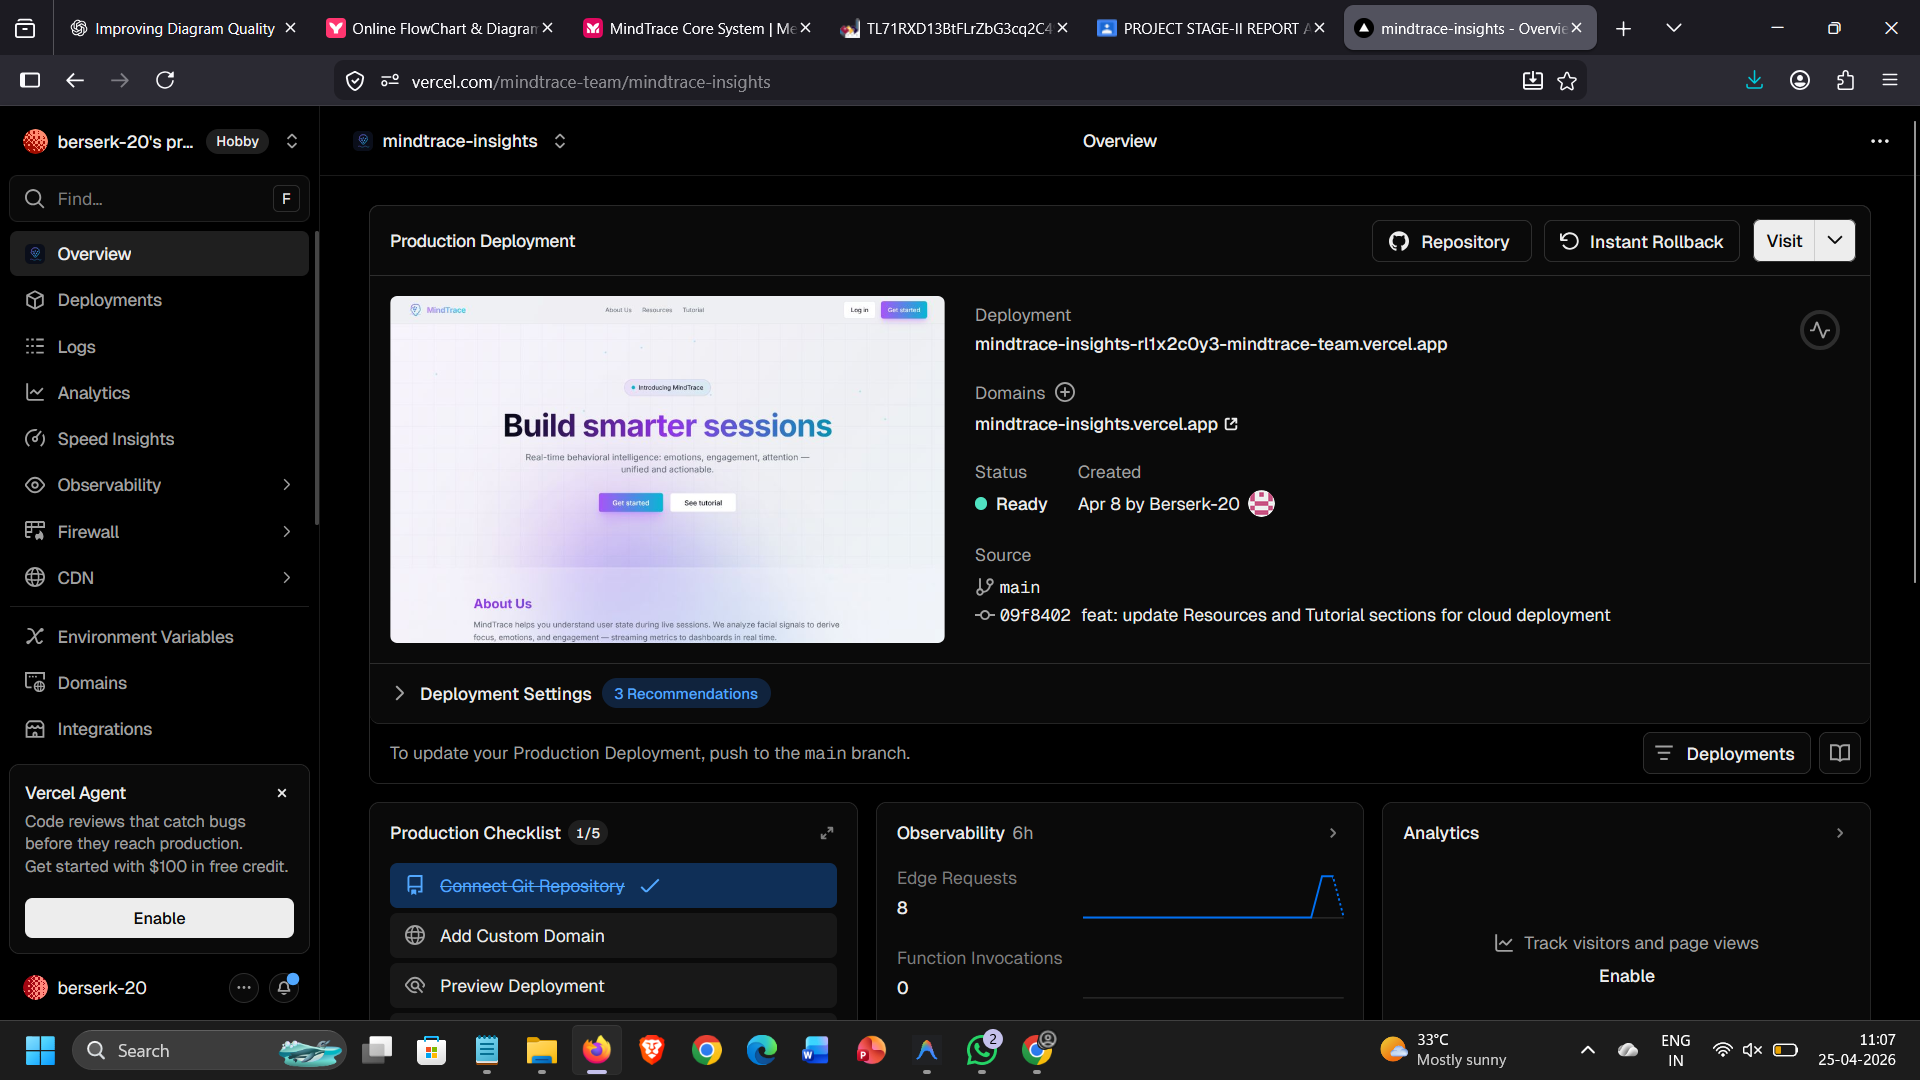
\includegraphics[width=\textwidth]{ss_vercel}
    \caption{Frontend Hosting on Vercel}
\end{subfigure}
\hfill
\begin{subfigure}[b]{0.48\textwidth}
    \centering
    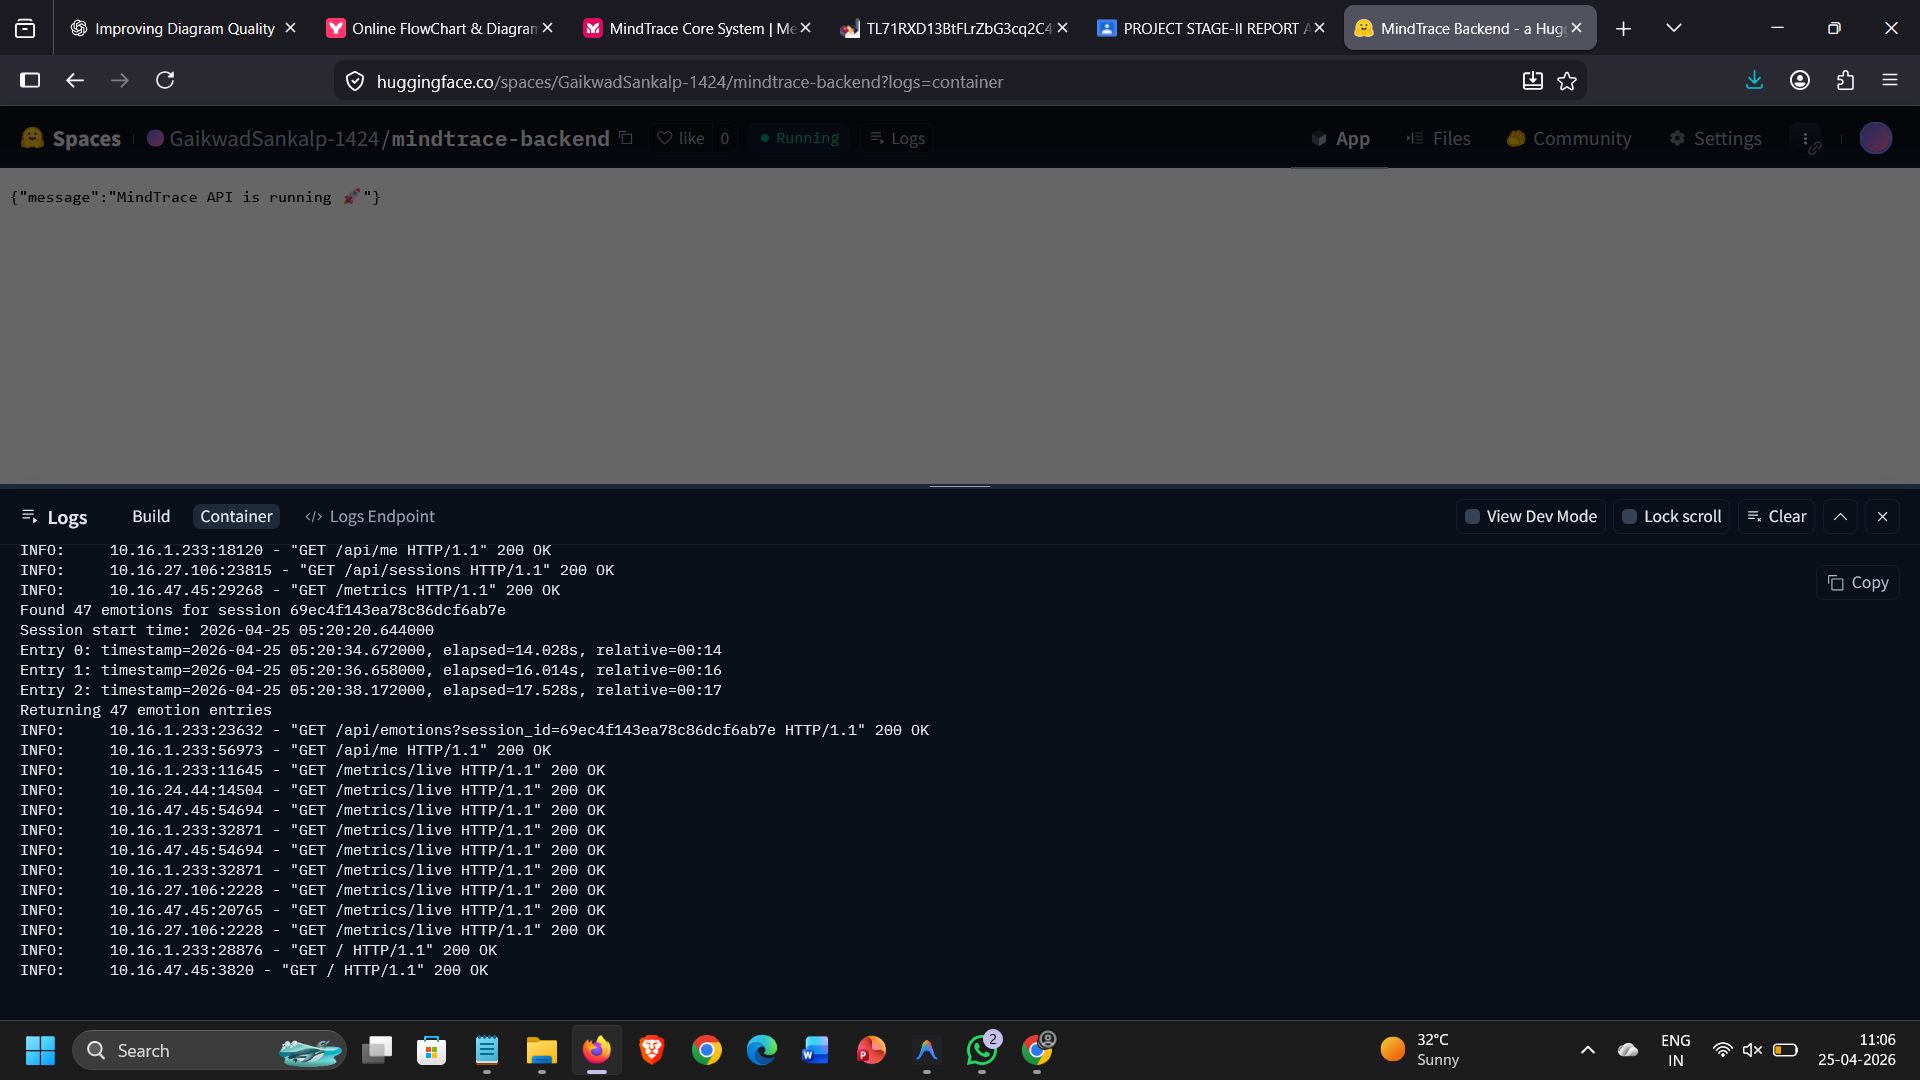
\includegraphics[width=\textwidth]{ss_huggingface}
    \caption{Backend API on Hugging Face}
\end{subfigure}
\caption{Cloud Deployment Infrastructure}
\label{fig:deployment}
\end{figure}

The session data is persisted in a MongoDB Atlas cluster, as shown in Figure
\ref{fig:mongodb}, which allows for real-time data exploration and long-term
storage of student engagement records.

\begin{figure}[H]
\centering
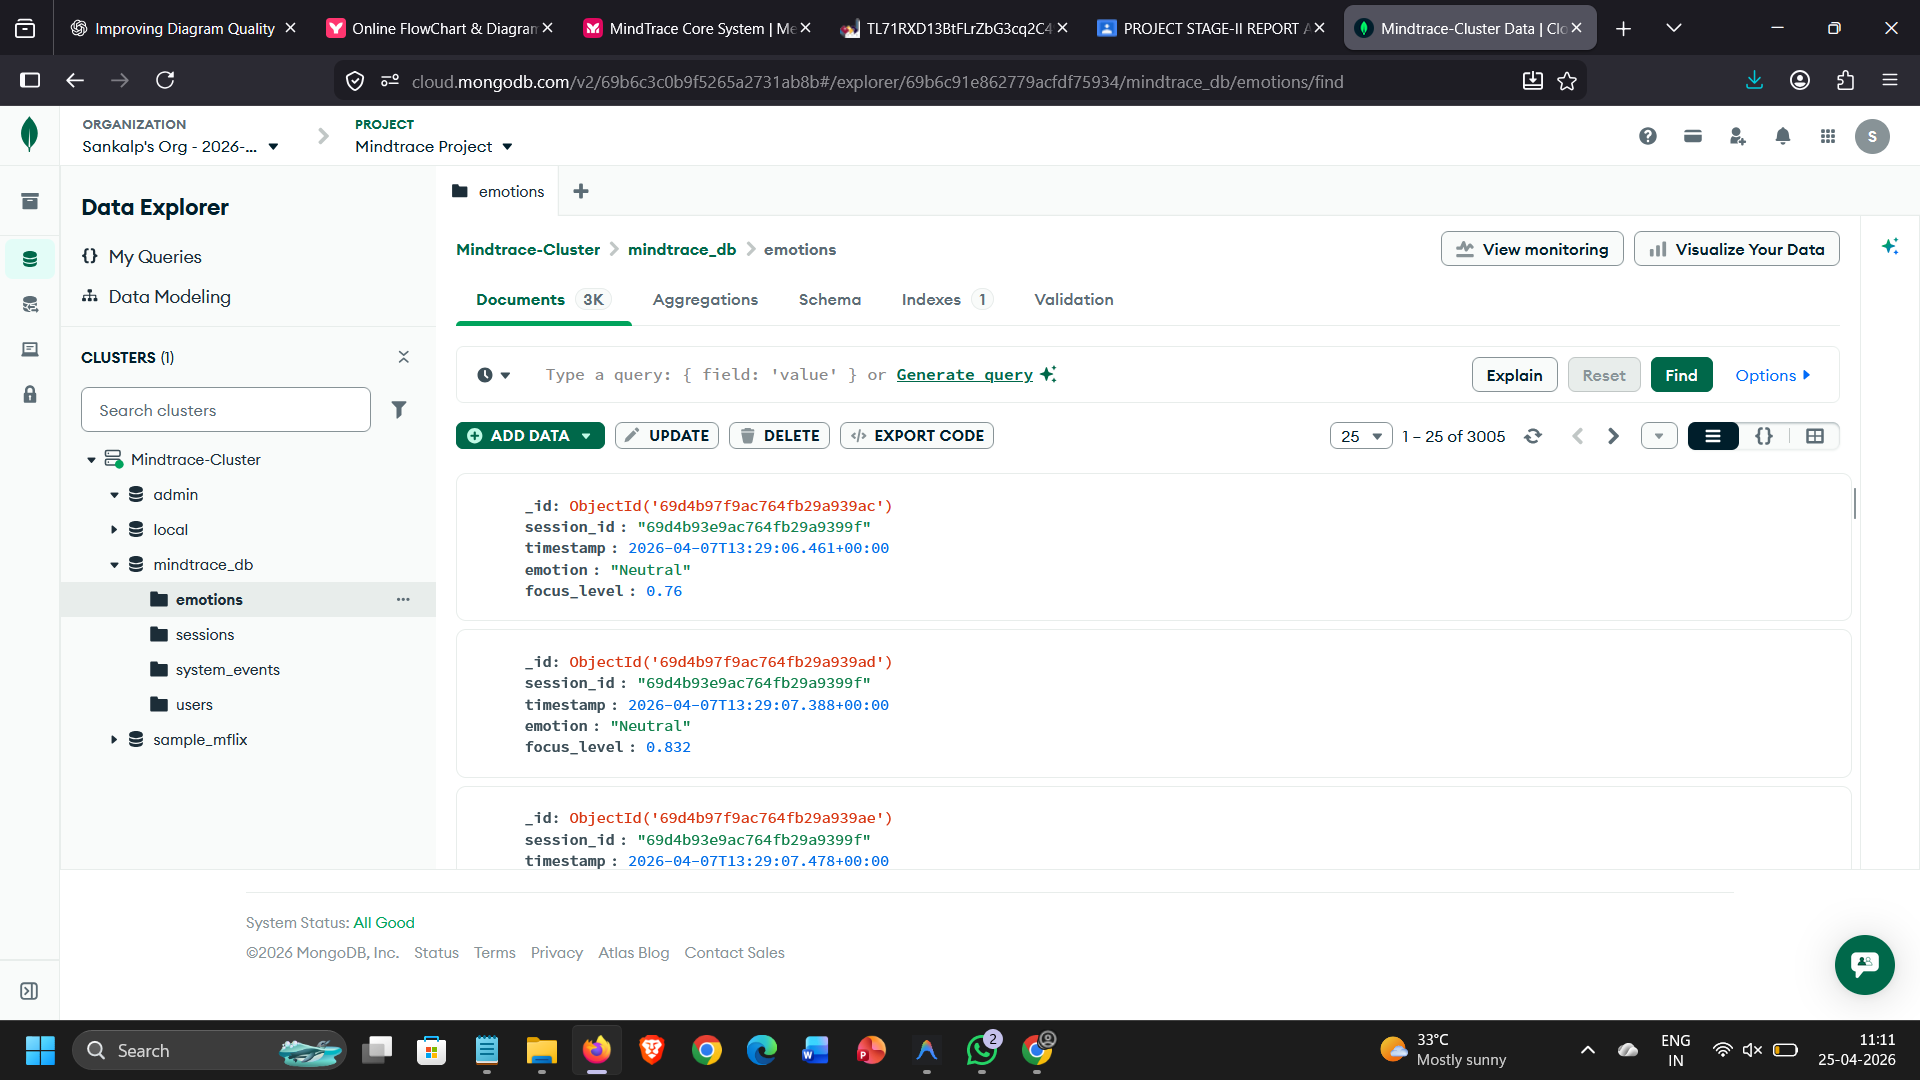
\includegraphics[width=0.85\textwidth]{ss_mongodb}
\caption{MongoDB Atlas Data Explorer (Session Records)}
\label{fig:mongodb}
\end{figure}

\section{Discussion}

\subsection{Achievement of Objectives}

All primary objectives defined in Chapter 1 were successfully achieved:

\begin{itemize}
    \item \textbf{Emotion classification}: Seven-class emotion detection
          with 85.7\% accuracy was implemented and deployed in real time.
    \item \textbf{Head pose and blink detection}: Accurately flags
          distraction events with a low false-positive rate.
    \item \textbf{Engagement scoring}: The composite score provides
          meaningful and interpretable feedback that correlates with
          observed participant behaviour.
    \item \textbf{Data persistence}: Session records are reliably stored
          and retrievable from MongoDB Atlas.
    \item \textbf{Dashboard}: A fully functional React dashboard with
          live overlays, charts, and admin panel was delivered.
    \item \textbf{Security}: JWT authentication and bcrypt password
          hashing were implemented and validated.
    \item \textbf{Cloud deployment}: The system is live and accessible
          via public URLs on Hugging Face Spaces and Vercel.
\end{itemize}

\subsection{Limitations}

\begin{itemize}
    \item The model exhibits reduced accuracy in low-lighting conditions,
          as the RAF-DB training images are primarily well-lit.
    \item \textit{Disgust} and \textit{Fear} classes have lower F1 scores
          due to underrepresentation in the dataset.
    \item The engagement score weights ($w_e$, $w_p$, $w_b$) were set
          empirically and may not generalise equally across all demographic
          groups.
    \item The single-instance deployment limits concurrent user capacity
          to approximately 20 users.
\end{itemize}

% ============================================================
%  CHAPTER 9 — CONCLUSION AND FUTURE SCOPE
% ============================================================
\chapter{Conclusion}

\section{Conclusion}

This project successfully designed, implemented, and deployed \textbf{MindTrace}
— a real-time emotion recognition and engagement tracking system that operates
entirely through a standard webcam without requiring any specialised hardware.
The system demonstrates that modern deep learning techniques can be effectively
applied to affective computing in educational and professional environments.

The key outcomes of the project are summarised as follows:

\begin{itemize}
    \item A \textbf{ResNet-18} model fine-tuned on the \textbf{RAF-DB} dataset
          achieved \textbf{85.7\% accuracy} in classifying seven emotional
          states, establishing a strong foundation for real-time affective
          feedback.

    \item \textbf{MediaPipe Face Mesh} enabled robust, landmark-based face
          detection that operates reliably at real-time frame rates without
          a GPU on the client side.

    \item The composite \textbf{engagement scoring algorithm} — combining
          emotional state, head pose estimation, and blink-rate analysis —
          produced scores that accurately reflected participant behaviour
          under controlled and real-world conditions.

    \item A \textbf{stateless FastAPI backend} deployed on Hugging Face Spaces
          demonstrated cloud-native design principles, supporting concurrent
          access and enabling hardware-independent operation.

    \item A \textbf{React-based analytics dashboard} provided an intuitive
          interface for live monitoring, session history, and multi-user
          administration, validated through user acceptance testing with an
          overall score of \textbf{4.2 out of 5}.

    \item The system \textbf{meets all functional and non-functional
          requirements} defined in the SRS, including the 300 ms latency
          target, HTTPS security, role-based access control, and
          cross-browser compatibility.
\end{itemize}

MindTrace bridges the gap between affective computing research and practical,
deployable applications. By providing objective, continuous engagement feedback,
it offers educators, corporate trainers, and researchers a powerful tool for
understanding how people interact with digital learning environments — without
the need for wearable sensors, invasive monitoring, or manual observation.

\section{Future Scope}

While MindTrace achieves its defined objectives, several directions remain
open for further enhancement:

\begin{enumerate}
    \item \textbf{Multi-person Monitoring}: Extending the system to track
          multiple faces simultaneously within a single frame would enable
          classroom-level engagement monitoring, where a single camera
          covers all participants.

    \item \textbf{Larger and More Diverse Datasets}: Training on a more
          diverse dataset — such as AffectNet (450,000+ images) or a
          combination of RAF-DB and CK+ — could improve model robustness
          across different ethnicities, ages, and lighting conditions.

    \item \textbf{Temporal Emotion Modelling}: Incorporating temporal
          context using \textbf{LSTM} or \textbf{Transformer-based}
          sequence models could capture dynamic emotional transitions
          more accurately than frame-level classification alone.

    \item \textbf{Voice and Physiological Fusion}: Integrating audio
          sentiment analysis (tone of voice) or physiological signals
          (heart rate via remote photoplethysmography) could produce a
          more holistic and accurate engagement metric.

    \item \textbf{On-Device Inference}: Optimising the ResNet-18 model
          using \textbf{quantisation} or \textbf{knowledge distillation}
          and deploying it as a \textbf{TensorFlow.js} model in the browser
          would eliminate network latency entirely and improve privacy by
          keeping all processing client-side.

    \item \textbf{Personalised Engagement Baselines}: Rather than using
          fixed score weights, the system could \textbf{learn individualised
          engagement baselines} over time using online learning, adapting
          to each user's natural expression and attention patterns.

    \item \textbf{LMS Integration}: Integrating MindTrace with popular
          Learning Management Systems such as \textbf{Moodle} or
          \textbf{Google Classroom} via APIs would allow engagement data
          to be linked directly to course content and assessment performance.

    \item \textbf{Scalable Deployment}: Deploying the backend on a
          container orchestration platform such as \textbf{Kubernetes}
          with auto-scaling would remove the current single-instance
          concurrency limitation and support large-scale institutional
          deployments.
\end{enumerate}

In summary, MindTrace lays a solid foundation for intelligent, non-invasive
engagement monitoring. Its modular, cloud-native architecture ensures that
each of the above enhancements can be adopted incrementally without
requiring a complete redesign of the system.

% ============================================================
%  REFERENCES
% ============================================================
\chapter{References}
\thispagestyle{plain}

\begin{enumerate}

\item K. Zhang, Z. Zhang, Z. Li, and Y. Qiao, ``Joint face detection and
alignment using multitask cascaded convolutional networks,''
\textit{IEEE Signal Processing Letters}, vol.\ 23, no.\ 10,
pp.\ 1499--1503, Oct.\ 2016.

\item S. Li, W. Deng, and J. Du, ``Reliable crowdsourcing and deep
locality-preserving learning for expression recognition in the wild,''
in \textit{Proc.\ IEEE Conf.\ Computer Vision and Pattern Recognition
(CVPR)}, Honolulu, HI, USA, 2017, pp.\ 2852--2861.

\item K. He, X. Zhang, S. Ren, and J. Sun, ``Deep residual learning for
image recognition,'' in \textit{Proc.\ IEEE Conf.\ Computer Vision and
Pattern Recognition (CVPR)}, Las Vegas, NV, USA, 2016, pp.\ 770--778.

\item V. Bazarevsky, Y. Kartynnik, A. Vakunov, K. Raveendran, and
M. Grundmann, ``BlazeFace: Sub-millisecond neural face detection on
mobile GPUs,'' \textit{arXiv preprint arXiv:1907.05047}, 2019.

\item Y. Wang, X. Li, D. Song, T. Li, B. Luo, and T. Liu,
``Suppressing uncertainties for large-scale facial expression recognition,''
in \textit{Proc.\ IEEE Conf.\ Computer Vision and Pattern Recognition
(CVPR)}, 2020, pp.\ 6897--6906.

\item Z. Zhao, Q. Liu, and F. Zhou, ``Robust lightweight facial expression
recognition network with label distribution training,'' in \textit{Proc.\
AAAI Conf.\ Artificial Intelligence}, 2021, vol.\ 35, pp.\ 3510--3519.

\item Z. Zhao, Q. Liu, G. Wang, ``Learning deep global multi-scale and
local attention features for facial expression recognition in the wild,''
\textit{IEEE Trans.\ Image Processing}, vol.\ 30, pp.\ 6544--6556, 2021.

\item C. D. Busso, M. Bulut, C. C. Lee, A. Kazemzadeh, E. Mower,
S. Kim, J. N. Chang, S. Lee, and S. S. Narayanan, ``IEMOCAP: Interactive
emotional dyadic motion capture database,'' \textit{Language Resources and
Evaluation}, vol.\ 42, no.\ 4, pp.\ 335--359, 2008.

\item A. Mollahosseini, B. Hasani, and M. H. Mahoor, ``AffectNet: A
database for facial expression, valence, and arousal computing in the wild,''
\textit{IEEE Trans.\ Affective Computing}, vol.\ 10, no.\ 1, pp.\ 18--31,
Jan.\ 2019.

\item P. Ekman and W. V. Friesen, ``Constants across cultures in the face
and emotion,'' \textit{Journal of Personality and Social Psychology},
vol.\ 17, no.\ 2, pp.\ 124--129, 1971.

\item T. Baltrusaitis, A. Zadeh, Y. C. Lim, and L. P. Morency,
``OpenFace 2.0: Facial behavior analysis toolkit,'' in \textit{Proc.\
13th IEEE Int.\ Conf.\ Automatic Face and Gesture Recognition (FG 2018)},
Xi'an, China, 2018, pp.\ 59--66.

\item S. Tiong, Y. Aris, and F. Hassan, ``Emotion recognition using ResNet
and LSTM for E-learning,'' in \textit{Proc.\ Int.\ Conf.\ Electrical
Engineering and Informatics (ICEEI)}, 2019, pp.\ 481--484.

\item FastAPI Documentation, ``FastAPI: Modern, fast (high-performance)
web framework for building APIs with Python,''
\url{https://fastapi.tiangolo.com}, accessed April 2026.

\item Meta Open Source, ``React --- A JavaScript library for building
user interfaces,'' \url{https://react.dev}, accessed April 2026.

\item Google, ``MediaPipe Face Mesh,''
\url{https://developers.google.com/mediapipe/solutions/vision/face_landmarker},
accessed April 2026.

\item ``A survey of deep learning-based facial expression recognition research,'' \textit{IEEE Affective Computing Journal}, 2023.

\item ``Improved facial emotion recognition model based on a novel deep network,'' \textit{Elsevier Computer Vision Letters}, 2024.

\item ``Advancements in driver fatigue detection: Comprehensive analysis of eye movement and facial-feature approaches,'' \textit{Springer Pattern Recognition and Image Analysis}, 2024.

\item ``Non-invasive fatigue detection and human–machine interaction via facial parameters,'' \textit{ACM Transactions on Human–Computer Interaction}, 2025.

\item ``Fatigue monitoring using wearables and AI,'' \textit{IEEE Sensors Journal}, 2025.

\end{enumerate}

% ============================================================
%  ANNEXURE  — custom title command
%  Mimics the numbered-chapter style: title vertically centred
%  on its own page, content begins on the NEXT page.
% ============================================================
\newcommand{\annexuretitle}[1]{%
  \clearpage
  \thispagestyle{plain}%
  \vspace*{\fill}
  {\centering
    \normalfont\Large\bfseries
    \MakeUppercase{#1}\par
  }%
  \vspace*{\fill}
  \addcontentsline{toc}{chapter}{#1}%
  \clearpage
  \thispagestyle{fancy}%
}

% ── Annexure - A ─────────────────────────────────────────────
\annexuretitle{Annexure - A}

\begin{singlespacing}\small

\section*{API Endpoint Reference}
\vspace{-0.5em}
\begin{table}[H]
\centering
\caption{MindTrace REST API Endpoints}
\renewcommand{\arraystretch}{1.1}
\begin{tabular}{lllp{4.5cm}}
\toprule
\textbf{Method} & \textbf{Endpoint}       & \textbf{Auth} & \textbf{Description} \\
\midrule
POST   & \texttt{/register}          & No    & Register a new user account \\
POST   & \texttt{/login}             & No    & Login and receive JWT token \\
POST   & \texttt{/api/analyze}       & Yes   & Submit webcam frame for analysis \\
POST   & \texttt{/api/session/start} & Yes   & Create a new session record \\
POST   & \texttt{/api/session/end}   & Yes   & Finalise and save current session \\
GET    & \texttt{/api/sessions}      & Yes   & Retrieve current user's sessions \\
GET    & \texttt{/api/admin/users}   & Admin & Retrieve all user records \\
GET    & \texttt{/api/admin/sessions}& Admin & Retrieve all sessions (all users) \\
\bottomrule
\end{tabular}
\end{table}

\vspace{0.3em}
\section*{Sample API Request and Response}
\vspace{-0.3em}
\textbf{Request} — POST \texttt{/api/analyze}:
\vspace{-0.5em}
\begin{verbatim}
{
  "frame": "<base64-encoded JPEG string>",
  "session_id": "6614f3a2c3e4b12a9d7f0011"
}
\end{verbatim}
\vspace{-1em}
\textbf{Response}:
\vspace{-0.5em}
\begin{verbatim}
{
  "emotion": "Happy",
  "confidence": 0.91,
  "engagement_score": 87,
  "head_pose": {
    "pitch": -2.3,
    "yaw":    4.1,
    "roll":   1.8
  },
  "blink_rate": 14
}
\end{verbatim}

\end{singlespacing}

% ── Annexure - B ─────────────────────────────────────────────
\annexuretitle{Annexure - B}

\section*{Technology Stack Summary}

\begin{table}[H]
\centering
\caption{Complete Technology Stack}
\begin{tabular}{lll}
\toprule
\textbf{Layer}        & \textbf{Technology}         & \textbf{Version} \\
\midrule
ML Framework          & PyTorch + torchvision       & 2.x \\
Model Architecture    & ResNet-18 (fine-tuned)      & --- \\
Face Detection        & MediaPipe Face Mesh         & 0.10+ \\
Computer Vision       & OpenCV                      & 4.x \\
API Framework         & FastAPI + Uvicorn           & 0.110+ \\
Database              & MongoDB Atlas + Motor       & 6.x \\
Authentication        & PyJWT + bcrypt              & --- \\
Frontend Framework    & React + Vite                & 18.x / 5.x \\
Charting Library      & Recharts                    & 2.x \\
HTTP Client           & Axios                       & 1.x \\
Backend Deployment    & Hugging Face Spaces (Docker)& --- \\
Frontend Deployment   & Vercel                      & --- \\
Version Control       & Git + GitHub                & --- \\
\bottomrule
\end{tabular}
\end{table}

\section*{Emotion Score Weights}

The engagement score is computed using the following empirically determined
weights applied to the three signal components:

\begin{table}[H]
\centering
\caption{Engagement Score Component Weights}
\begin{tabular}{lcc}
\toprule
\textbf{Component}     & \textbf{Weight} & \textbf{Rationale} \\
\midrule
Emotion score ($S_e$)  & 0.50            & Primary indicator of cognitive state \\
Head pose score ($S_p$)& 0.35            & Strong proxy for visual attention \\
Blink rate score ($S_b$)& 0.15          & Supplementary fatigue indicator \\
\midrule
\textbf{Total}         & \textbf{1.00}   & --- \\
\bottomrule
\end{tabular}
\end{table}

% ── Annexure - C ─────────────────────────────────────────────
\annexuretitle{Annexure - C}

\section*{Plagiarism Report}

The following pages contain the plagiarism check report generated for this
project document, confirming the originality of the submitted work.

\vspace{0.5em}

\begin{figure}[H]
  \centering
  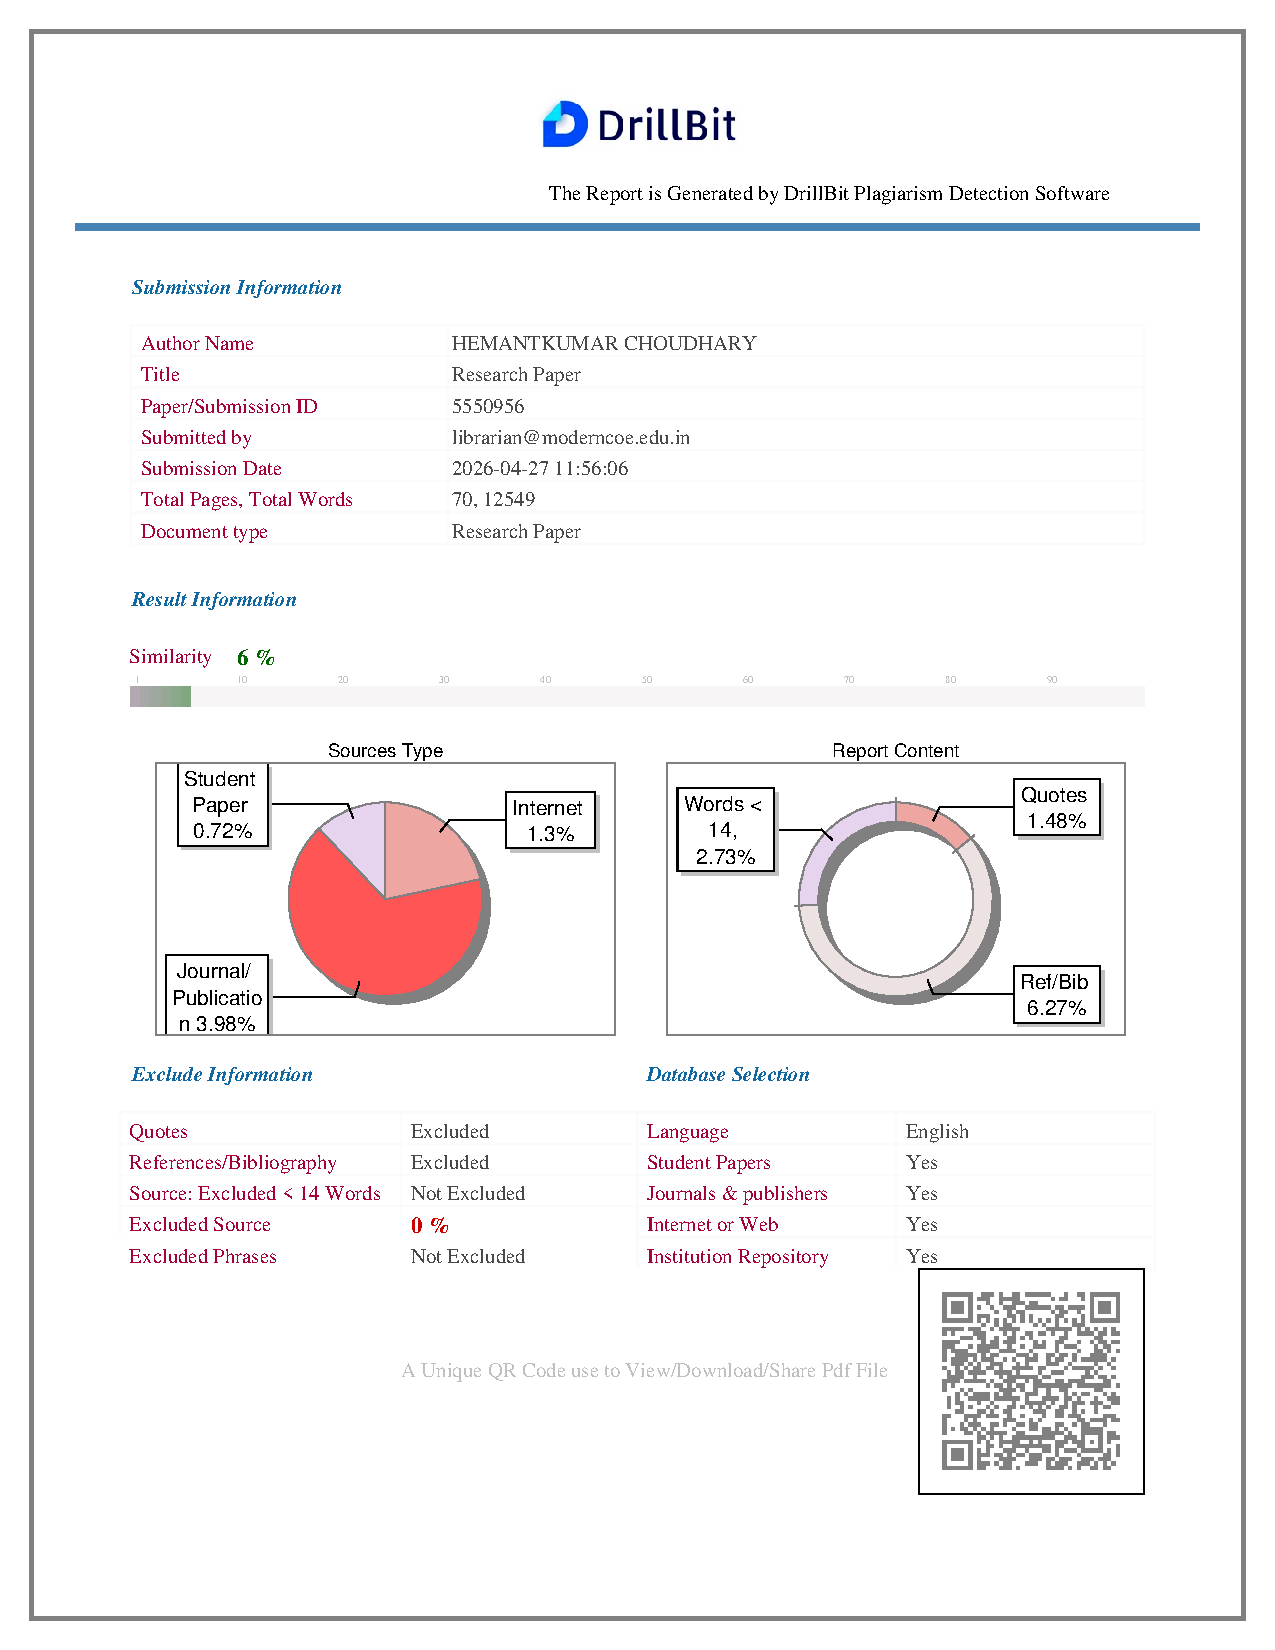
\includegraphics[page=1,width=0.85\linewidth,keepaspectratio]{Plagiarism Report 1.pdf}
  \caption[]{Plagiarism Report Page 1}% suppress auto LOF entry
\end{figure}
\addcontentsline{lof}{figure}{Plagiarism Report Page 1}% manual unnumbered LOF entry

\newpage
\begin{figure}[H]
  \centering
  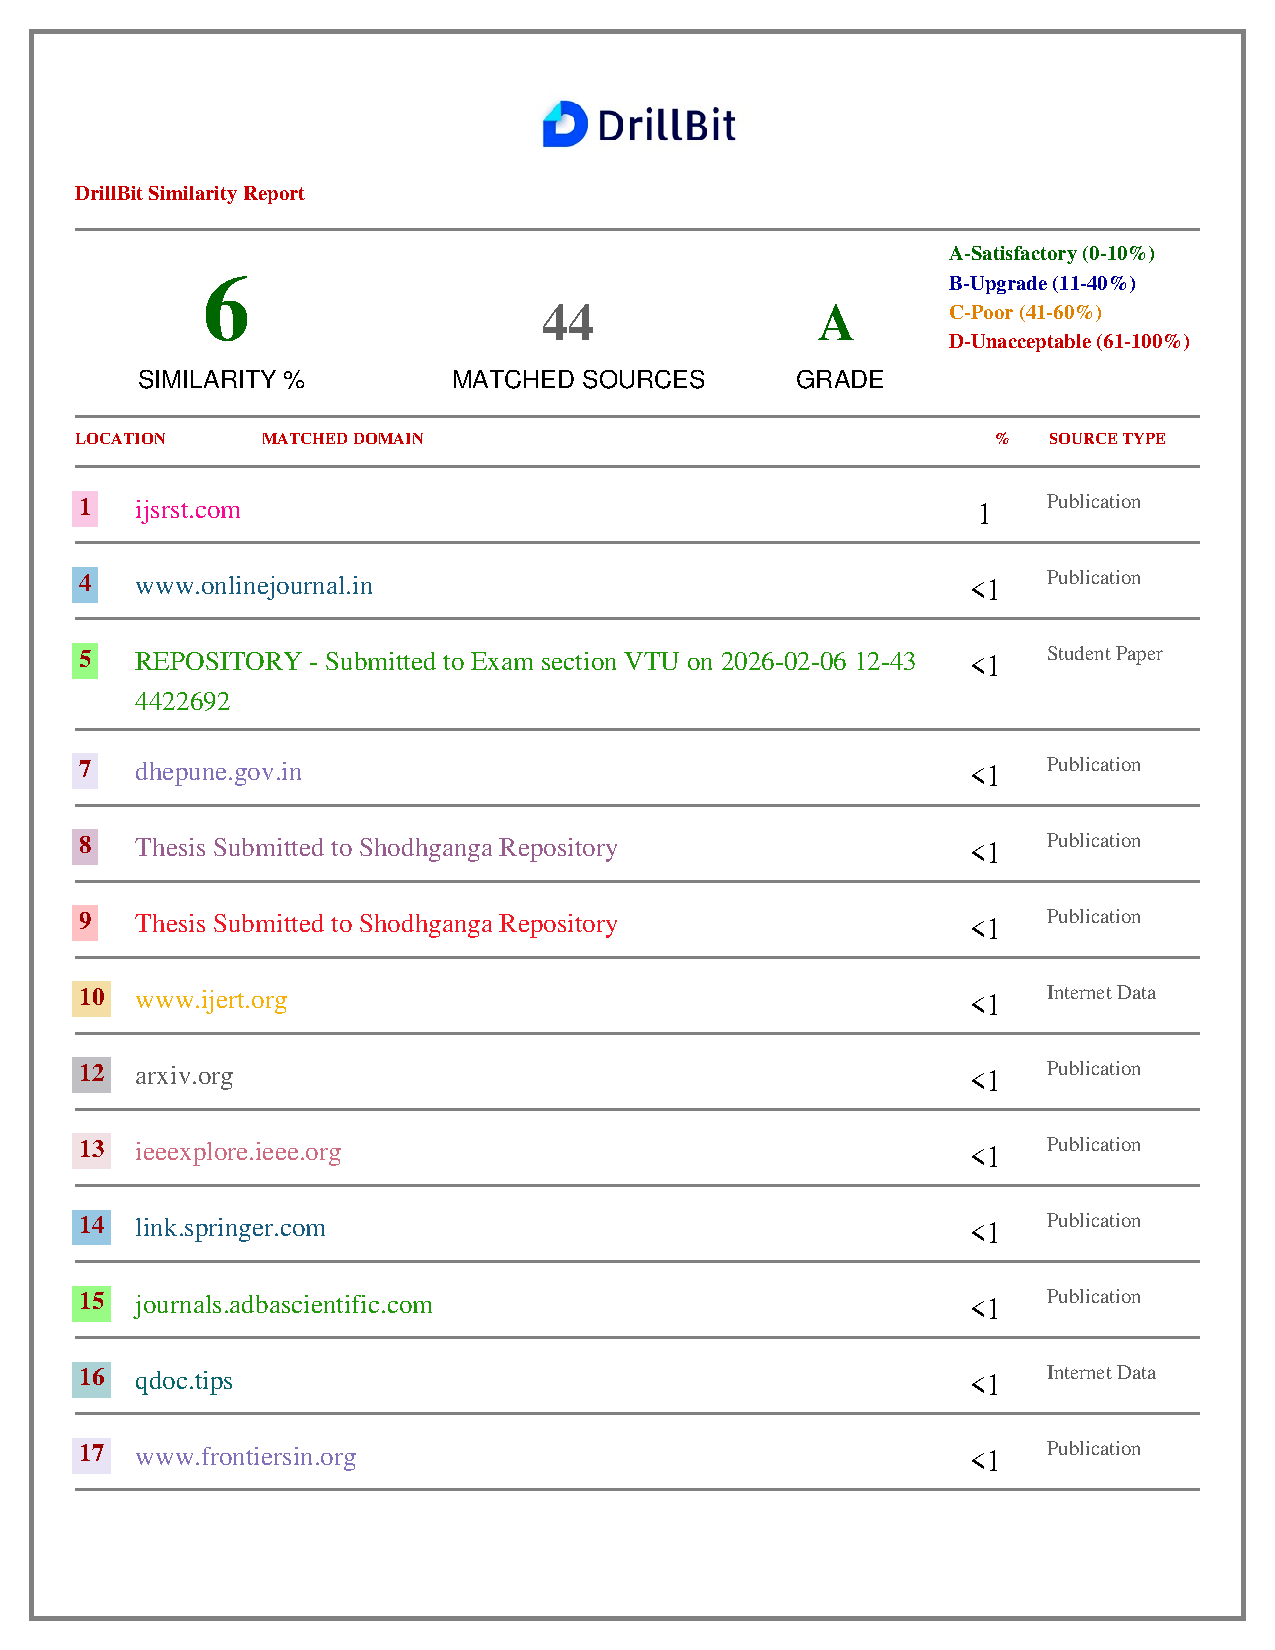
\includegraphics[page=1,width=0.85\linewidth,keepaspectratio]{Plagiarism Report 2.pdf}
  \caption[]{Plagiarism Report Page 2}% suppress auto LOF entry
\end{figure}
\addcontentsline{lof}{figure}{Plagiarism Report Page 2}% manual unnumbered LOF entry


\end{document}
